%% 
%% Master Thesis
%% Autor: Martin Wichmann
%% 
%% TODO:
%% - Danksagung
%% - NDA/IP klären!!! (VW, EB, evtl. dSPACE?!)
%% - steuernde Komponente oder Steuerungskomponente
%% - netzwerk-management oder netzwerkmanagment


\documentclass[
  a4paper,					    % a4paper (sic!)
  %oneside,
  twoside,
  DIV=calc,     				% KOMA-Script soll den optimalen Satzspiegel berechnen
  bibliography=totoc,
  %abstracton,  				% Überschrift der Zusammenfassung aktivieren
  cleardoublepage=empty,
  ngerman,     					% allen Paketen die Hauptsprache mitteilen
  %draft       					% draft version  
  final       					% final version
]{scrbook}	
%%%%%%%%%%%%%%% Grundlegendes %%%%%%%%%%%%%%%
\usepackage[utf8]{inputenc}
\usepackage[T1]{fontenc}
\usepackage[english,ngerman]{babel} 	% Unterstuezung fuer englisch und deutsch
\usepackage{setspace}			% erlaubt 1 1/2 fachen Zeilenabstand
%%%%%%%%%%%%%%% Tabellen %%%%%%%%%%%%%%%
\usepackage{lscape}
\usepackage{booktabs}			% \toprule, \midrule und \bottomrule in Tabellen
\usepackage{multirow}
\usepackage{paralist}
%%%%%%%%%%%%%%% Mathe %%%%%%%%%%%%%%%
%\usepackage{amsmath, amsthm, amscd, amssymb, amsfonts}
%%%%%%%%%%%%%%% Typografie %%%%%%%%%%%%%%%
\usepackage{ellipsis}			% fix uneven spacing around ellipses in LaTeX text mode.
\usepackage{microtype} 			% optischer Randausgleich (font expansion and character protrusion)
%%%%%%%%%%%%%%% Schriften %%%%%%%%%%%%%%%
\usepackage{lmodern}
%%%%%%%%%%%%%%% Sonstiges %%%%%%%%%%%%%%%
\usepackage{scrhack}            % KOMA Paket um zusammenarbeit mit anderen Paket (listings) zu verbessern
\usepackage{listings}			% Code-Abschnitt mit Syntax-Highlighting
\lstset{
    language=C,
    breaklines=true,
    breakatwhitespace=true
    basicstyle=\footnotesize,
    numbers=left,
    numberstyle=\footnotesize,
    stepnumber=1,
    numbersep=5pt,
    extendedchars=true,
    inputencoding=utf8,
    breakindent=30pt,
    escapeinside={\%(}{\%)},
    captionpos=b
}
%%%%%%%%%%%%%%% Grafiken %%%%%%%%%%%%%%%
\usepackage[pdftex]{graphicx}	% das pdftex soll das Handling von Bildern verbessern
\graphicspath{{images/}}		% Bilder im Verzeichnis images suchen
\usepackage{tikz}
\usepackage{wrapfig}
\usepackage{caption}            % Von subcaption benötigt
\usepackage{subcaption}         % Subabbildungen
\usepackage{pgfgantt}           % pgf verwenden um Gantt Diagramme zu erstellen (http://www.ctan.org/pkg/pgfgantt)
\usepackage{rotating} 			% fuer gedrehte Tabellen und Bilder
\usepackage[
    pdftex,
    bookmarks, bookmarksopen, bookmarksopenlevel=1, bookmarksnumbered=true,
    pdfpagemode={UseNone},		% UseNone, FullScreen, UseThumbs, UseOutlines, (UseOC, UseAttachments)
    pdfpagelayout={TwoPageRight},	% SinglePage, OneColumn, TwoColumnLeft, TwoColumnRight, TwoPageLeft, TwoPageRight
    plainpages=false, 
    pdfkeywords={AUTOSAR, Virtualisierung, ECU, Python, CAN},
    pdfsubject={Virtualisierung von AUTOSAR Softwarekomponenten für die Erprobung},
    pdftitle={Virtualisierung von AUTOSAR Softwarekomponenten für die Erprobung},
    pdfauthor={Martin Wichmann},
]{hyperref}
%%%%%%%%%%%%%%% Zitieren und Index %%%%%%%%%%%%%%%
\usepackage[numbers]{natbib}
\usepackage[order=word, toc, acronym, nonumberlist]{glossaries} % Glossar und Liste der Akronyme
\makeglossaries
\loadglsentries{acronym}
\loadglsentries{glossary}
%%%%%%%%%%%%%%%%%%%%%%%%%%%%%%%%%%%%%%%%%%%%%%%%%%%%

%%%%%%%%%%%%%%%%%%%%%%%% Eigene Definitionen %%%%%%%%%%%%%%%%%%%%%%%%%%%%%%

% Hack um die Underful Hbox Error in der Bibliography zu unterbinden
% Sollte keine Probleme machen, solange \sloppy nicht von Hand verwendet wird (sollte eh nicht!).
\usepackage{etoolbox}
\apptocmd{\sloppy}{\hbadness 10000\relax}{}{}

\addto{\captionsngerman}{\renewcommand*{\bibname}{Quellenverzeichnis}}

% Kommando für Klasse/Methoden in description enviroments
\newcommand{\apiitem}[1]{\item[\texttt{#1}] \hfill \\}

%%% Trennungen %%%%%%%%%%%%%%%%%%%%%%%%%%%%%%%%%%%%%%%%%%%
\hyphenation{Netz-werk-Ma-nage-ment}

%%% 1 1/2 fachen Zeilenabstand wählen %%%%%%%%%%%%%%%%%%%%
\onehalfspacing
\typearea[current]{calc}				% Neuberechnung des Satzspiegels

%%%%%%%%%%%%%%%%%%%%%%%%%%%% Begin document %%%%%%%%%%%%%%%%%%%%%%%%%%%%%%%
\begin{document}
\selectlanguage{ngerman}
\frontmatter

%%%%%%%%%%%%%%%%%%%%%%%%%%%%%%%%% Titel %%%%%%%%%%%%%%%%%%%%%%%%%%%%%%%%%%
\titlehead{\center{\large \textsc{Ostfalia Hochschule für angewandte Wissenschaften}}}
\subject{Masterarbeit}
\title{Virtualisierung von AUTOSAR Softwarekomponenten für die Erprobung}
\author{Martin Wichmann\\Matrikel 701\,277\,37}
\date{Eingereicht am TODO}
\publishers{Prüfer: 

  Prof. Dr.-Ing. Gert Bikker

  Prof. Dr.-Ing. Jürgen Kreyßig

  }

\lowertitleback{Diese Arbeit wurde mit Hilfe von Freier Software erstellt: \\
Gesetzt mit Hilfe von {\KOMAScript} und {\LaTeX}. Dia sowie PGF/Ti\emph{k}Z für die Erstellung der Grafiken und gedit als Editor. Xubuntu als offenes Betriebssystem. \\ \\ Diese Arbeit ist, falls nicht anders angegeben, freigegeben unter der Creative Commons BY-SA 3.0 Lizenz\cite{CCBYSA} und ist erreichbar unter: \url{https://github.com/erebos42/Documents/tree/master/Master_Thesis}.
}
\dedication{Einfachheit ist Voraussetzung für Zuverlässigkeit.\\ \vspace{1cm}
\textit{Edsger Wybe Dijkstra}
}



\begin{singlespace}
\maketitle

%%%%%%%%%%%%%%%% Abstract %%%%%%%%%%%%%%%%%%%%%%%


\section*{Zusammenfassung}
\pdfbookmark[1]{Zusammenfassung}{Zusammenfassung}
Nach fast zehn Jahren seit den ersten Bemühungen um AUTOSAR, haben sich die Architektur und die Entwicklungsmethoden mittlerweile in der Automobilindustrie etabliert. Diese Masterarbeit betrachtet die Möglichkeiten AUTOSAR Komponenten virtualisiert einzusetzen. Hierzu wird ein Fallbeispiel betrachtet, mit Hilfe dessen sowohl die Virtualisierung, inklusive der Kommunikation, als auch AUTOSAR selber evaluiert wird. Um den Bedarf an AUTOSAR-Entwicklern zu decken, wird an der Ostfalia Hochschule für angewandte Wissenschaften seit einige Jahren AUTOSAR in der Lehre eingesetzt. Um diese Bemühungen zu unterstützen soll diese Arbeit zusätzlich als Grundlagen-Einführung dienen.

\textbf{Schlüsselwörter}: AUTOSAR, eingebettete Virtualisierung, ISO 26262
\vfill

\foreignlanguage{english}{
\section*{Abstract}
After almost ten years since the beginning of AUTOSAR, the architecture and development process is established in the automotive industry. This master thesis looks at the possibilities to use virtualized AUTOSAR components. To do this a case study is examined to evaluate both the virtualization, including the communication, and AUTOSAR as a concept. To cover the demand for AUTOSAR developers, the Ostfalia Hochschule für angewandte Wissenschaften has placed AUTOSAR in its curriculum. To support these efforts, this thesis is written to cover the fundamentals of AUTOSAR.
}

\textbf{Keywords}: AUTOSAR, embedded virtualization, ISO 26262
\vfill

\thispagestyle{empty}

%%%%%%%%%%%%%%%%%%%%%%%%%%%%%% Verzeichnisse %%%%%%%%%%%%%%%%%%%%%%%%%%%%%%

\tableofcontents               	% Inhaltsverzeichnis
\listoffigures               		% Abbildungsverzeichnis
\listoftables             			% Tabellenverzeichnis
\lstlistoflistings          		% Listenverzeichnis
\end{singlespace}









%%%%%%%%%%%%%%%%%%%%%%%%%%%%%%% Einleitung %%%%%%%%%%%%%%%%%%%%%%%%%%%%%%%%%%
\mainmatter
\chapter{Einleitung}
\label{sec:Einleitung}
Die Möglichkeiten der Virtualisierung werden im Serverbereich bereits seit Jahren genutzt. Aber auch eingebettete Systeme können von diesen Techniken profitieren und damit die Anzahl der Steuergeräte vermindern und Kosten sparen. Vor allem eine steigende Komplexität und Umfang zwingen die Automobilindustrie zum Umdenken. An diesem Punkt setzt AUTOSAR an. Diese moderne Systemarchitektur erfährt seit einigen Jahren eine immer stärkere Verbreitung. 

Diese Masterarbeit betrachtet die Möglichkeiten der Virtualisierung im embedded Bereich anhand eines Fallbeispiels. In diesem Zusammenhang wird ebenfalls AUTOSAR näher untersucht und in die Virtualisierung eingebunden. Das betrachtete Fallbeispiel wird im folgenden Kapitel vorgestellt. Anschließend werden die theoretischen Grundlagen erläutert und diskutiert. Dabei werden die Themengebiete \emph{Virtualisierung} und \emph{AUTOSAR} betrachtet. Die in diesem Zusammenhang ebenfalls interessante funktionale Sicherheit nach \emph{ISO 26262} wird ebenso untersucht.

Im darauf folgenden Kapitel wird das Fallbeispiel und dessen Umsetzung vorgestellt. Dabei wird auf alle relevanten Punkte näher eingegangen. Die Ergebnisse des Fallbeispiels werden im letzten Kapitel analysiert, und untersucht ob die vorgestellten Techniken eine Zukunft in realen Projekten haben.




%%%%%%%%%%%%%%%%%%%%%%%%%%%%%%% Vorstellung Fallbeispiel %%%%%%%%%%%%%%%%%%%%%%%%%%%%%%%%%%
\chapter{Motivation und Planung}
\label{sec:MotivationPlanung}
Das in dieser Masterarbeit betrachtete Praxisbeispiel ist eine Scheinwerfersteuerung inklusive User-Interface. Dies ist bewusst als minimales Beispiel konzipiert, um den Fokus auf die Virtualisierung und Evaluierung zu legen.

\begin{figure}[ht]
    \centering
    \input{./images/arch_begin.dia}
    \caption{Vorläufige Architektur}
    \label{fig:arch_begin}
\end{figure}

Die geplante Architektur der Scheinwerfersteuerung ist in Abbildung \ref{fig:arch_begin} zu sehen. Dabei sind zwei getrennte Hardwareelemente zu erkennen. Zum Einen das Scheinwerfersteuergerät und zum Anderen das in dieser Arbeit betrachtete steuernde System. Das Steuergerät übernimmt die direkte Steuerung der Scheinwerfer und ist per CAN-Bus mit dem anderen steuernden System verbunden.  Dieses beherbergt ein virtuelles AUTOSAR und Linux auf einem Windows Host.

Aus dieser Architekturbeschreibung lassen sich vier Kernbereiche dieser Masterarbeit ableiten:

\begin{itemize}
    \item Virtualisierung von AUTOSAR und Linux
    \item Entwicklung der AUTOSAR-Komponente
    \item Kommunikation zwischen Linux und AUTOSAR
    \item Kommunikation zwischen AUTOSAR und der Scheinwerfer-ECU (inklusive Netzwerkmanagement)
\end{itemize}

Hierbei ist zu beachten, dass das Aktivieren des Netzwerkmanagements erst möglich ist, sobald eine Kommunikation zwischen AUTOSAR und der Hardware möglich ist.

Da der Zeitaufwand für die einzelnen Phasen zu Beginn nur sehr schwer einzuschätzen ist, wird für jede Phase des Projektes der Zeitraum eines Monats vorgesehen. Dazu kommen noch ein Monat Evaluation und Sicherheitsbetrachtung des Systems und zum Schluss ein Monat Fertigstellen der schriftlichen Arbeit. Die Zeitplanung ist in einem Gantt-Diagramm in Abbildung \ref{fig:gantt} zu sehen. Jede Phase enthält die Vorbereitung, Umsetzung und Dokumentation des entsprechenden Bereichs.

% TODO: Das Diagramm sieht irgendwie nicht gut aus...
\begin{figure}[ht]
    \centering

    \begin{ganttchart}{12}
    \gantttitle{2012}{8} 
    \gantttitle{2013}{4} \\
    \gantttitlelist{9,10,11,12,1,2}{2} \\
    \ganttbar{Virtualisierung}{1}{2} \\
    \ganttbar{Kommunikation Linux/AUTOSAR}{3}{4} \\
    \ganttbar{Kommunikation AUTOSAR/ECU}{5}{6} \\
    \ganttbar{AUTOSAR Komponente}{7}{8} \\
    \ganttbar{Evaluation}{9}{10} \\
    \ganttbar{Fertigstellen der Arbeit}{11}{12} 
    \end{ganttchart}

    \caption{Zeitplanung Masterarbeit}
    \label{fig:gantt}
\end{figure}


%%%%%%%%%%%%%%%%%%%%%%%%%%%%%%% Grundlagen %%%%%%%%%%%%%%%%%%%%%%%%%%%%%%%%%%
\chapter{Grundlagen}
\label{sec:Grundlagen}
Dieses Kapitel enthält Grundlagen zu den Themen AUTOSAR und Virtualisierung. Dabei wird AUTOSAR ausführlich betrachtet, da es sich dabei um ein extrem umfangreiches Thema handelt. Speziell die Kommunikations-Konzepte, realisiert durch Virtual-Functional-Bus und Runtime-Enviroment, werden in den Fokus gelegt. Zusätzlich ist dieser Teil der Arbeit als Einführung in AUTOSAR zu sehen. Dadurch soll der Einstieg für zukünftige Arbeiten erleichtert werden.


%%%%%%%%%%%%%%%%%%%%%%%%%%%%%%% Virtualisierung %%%%%%%%%%%%%%%%%%%%%%%%%%%%%%%%%%
\section{Virtualisierung}
\label{sec:Virtualisierung}
Der Begriff \emph{Virtualisierung} bezeichnet eine Reihe von Techniken, die verwendet werden, um die Ressourcen eines Rechner-Systems zu verwalten. Hierdurch kann ein reales System, auf mehrere virtuelle Systeme aufgeteilt, und als solche genutzt werden. Dabei können verschiedene Ziele im Vordergrund stehen. Im Bereich der Virtualisierung wird dass System, dass den Hypervisor ausführt Host genannt. Ein Gastsystem hingegen, wird vom Hypervisor verwaltet.

Aus dem Desktopbereich ist die Systemvirtualisierung bekannt, wie sie zum Beispiel mittels VirtualBox\footnote{VirtualBox zu finden unter \url{www.virtualbox.org}} umgesetzt ist. Hierbei werden die Ressourcen des bestehenden Systems durch einen Hypervisor, auch Virtual Machine Monitor (kurz VMM) genannt, verwaltet und den virtuellen Instanzen zugeordnet. Diese Variante wird vor allem eingesetzt, um Zugriff auf einen anderes Betriebssystem zu erhalten, um so spezielle Software ausführen zu können.

Im Gegensatz dazu wird im Serverbereich der Fokus auf andere Bereiche gelegt. Die hier verfolgten Ziele sind vor allem eine einfache Wartbarkeit, Ausfallsicherheit und Ressourcenschonung. Mittels virtueller Server können Ausfallzeiten minimiert werden, indem bei einem Hardware-Ausfall die VM auf eine andere Hardware ausgelagert werden kann.

Virtualisierung kann mittels einer Reihe von Techniken realisiert werden. Hier wird unterschieden, ob die Hardware direkt zum Gastsystem weitergegeben wird, oder aber eine eigene virtuelle Hardware emuliert wird. Außerdem könnte ein Gastsystem Teile des Hosts, zum Beispiel dessen Kernel, mitverwenden. Klassischerweise werden Hypervisoren in zwei Kategorien eingeteilt (vgl. \cite[Seite 22 ff.]{hypervisor}). Diese Einteilung stimmt nicht ganz mit der Praxis überein, da der Übergang zwischen Hypervisor und Betriebssystem fließend verläuft. Für die folgenden Betrachtungen soll diese Einteilung jedoch genügen.

\begin{figure}
    \centering
    \begin{subfigure}[b]{0.49\textwidth}
        \centering
        \input{./images/virt_type1.dia}
        \caption{Type 1-Hypervisor}
        \label{fig:hypervisor_type1}
    \end{subfigure}
    \begin{subfigure}[b]{0.49\textwidth}
        \centering
        \input{./images/virt_type2.dia}
        \caption{Type 2-Hypervisor}
        \label{fig:hypervisor_type2}
    \end{subfigure}
    \caption{Hypervisor Kategorien}
    \label{fig:hypervisor}
\end{figure}

\paragraph{Type 1 (bare host)} Hierbei handelt es sich um native Hypervisoren, die direkt auf der Hardware lauffähig sind. Wie in Abbildung \ref{fig:hypervisor_type1} zu sehen ist, bauen diese auf kein Betriebssystem auf und verwalten selbstständig die Ressourcen und Gastsysteme. Aus diesem Grund sind sie vor allem interessant für eingebettete Systeme. Type 1-Hypervisoren werden genauer im nächsten Kapitel betrachtet.

\paragraph{Type 2 (extended host)} Ein Type 2-Hypervisor, sichtbar in Abbildung \ref{fig:hypervisor_type2}, ist nur auf einem vollständigen Betriebssystem lauffähig. Damit ist der Hypervisor eine logische Schicht zwischen dem Host und Gast und kann von den Vorteilen eines Betriebssystems profitieren. Hieraus ergibt sich, dass ein Type 2-Hypervisor meist kleiner und schneller ist.





%%%%%%%%%%%%%%%%%%%%%%%%%%%%%%% Embedded Virtualisierung %%%%%%%%%%%%%%%%%%%%%%%%%%%%%%%%%%
\section{Virtualisierung bei eingebetteten Systemen}
\label{sec:EVirtualisierung}
Virtualisierung im Bereich der eingebetteten Systeme, auch bekannt als \emph{Embedded Virtualization} und \emph{Time and Space Partitioning} (kurz TSP), hat in den letzten Jahren immer mehr an Bedeutung gewonnen. Da Mikrocontroller und SOCs\footnote{System-on-a-Chip, dt. Ein-Chip-System} immer leistungsfähiger werden und mehr Rechenkerne besitzen, ist es sinnvoll diese Leistung auszunutzen, um die Effektivität zu erhöhen und Kosten zu sparen. Gerade im Automobil-Bereich, in dem die Anzahl der Steuergeräte zum Teil auf mittlerweile über 50 innerhalb eines Autos gestiegen ist, kann es die Kosten erheblich reduzieren, wenn stattdessen einige dieser System virtualisiert werden können.

Hypervisor im embedded Bereich müssen bestimmte Anforderungen erfüllen die viele Hypervisoren nicht beachten. Zu diesen Anforderungen gehört ein geringer Energieverbrauch und effiziente Speichernutzung. Ein weiterer wichtiger Punkt ist die Echtzeitfähigkeit. Diese ist vor allem kritisch, da meist eine zweistufige Schedulerarchitektur entsteht, zum einen der Scheduler des Hypervisors und zum anderen der Scheduler des Gastsystems. Eine Echtzeitanalyse wird hierdurch verkompliziert (vgl. \cite{two_lvl_sched}).

Um nur ein einfaches Beispiel zu nennen, könnte ein Anwendung mit vier Subsystemen betrachtet werden. Diese Subsysteme könnten alle in ein einziges System mit einer 4-Kern CPU vereint und genauso wie vorher verwendet werden. Je nach benötigter Leistung könnte das resultierende System durchaus auch verkleinert und damit kostengünstiger gestaltet werden. Jedoch entstehen auch Probleme, wie ein Overhead durch den Hypervisor, durch den eine höhere Leistung nötig ist. Außerdem müssen natürlich alle nötigen Ein- und Ausgänge der Subsysteme auf dem resultierenden System vorhanden sein.

Die Vorteile eingebetteter Virtualisierung wurden bereits vor einiger Zeit erkannt und von einigen Bereichen der Industrie umgesetzt. In der Avionik ist diese Technik als \emph{Integrated Modular Avionics}, kurz IMA, bekannt und wird durch verschiedene Standards\footnote{Zum Beispiel Def Stan 00-74 der ASAAC und STANAG 4626 als NATO Standard.} beschrieben. Die aktuell wichtigste Spezifikation ist dabei die seit 1996 existierende \emph{ARINC 653}. Dabei handelt es sich um einen Standard für \emph{sichere, partitionierte Echtzeit-Systeme im Avionik-Bereich} (vgl. \cite{arinc653_wr}). Ein Ziel der Spezifikation ist die Verbesserung der Wiederverwendbarkeit, Portabilität und Modularität der eingesetzten Komponenten.

\begin{figure}[ht]
    \centering
    \input{./images/arinc653.dia}
    \caption[ARINC 653 Architektur Übersicht]{ARINC 653 Architektur Übersicht\cite{arinc653_wr}}
    \label{fig:arinc_653}
\end{figure}

Abbildung \ref{fig:arinc_653} zeigt einen Überblick über dieses System. Das Konzept besteht aus einem zugrunde liegendem Echtzeit-Betriebssystem, dass den darauf ausgeführten Softwareinstanzen die sogenannte APEX-API\footnote{APplication/EXecutive-API} anbietet. Diese ist auch eingeschränkt zu POSIX kompatibel (vgl. \cite{wiki:arinc_653}), wodurch auch POSIX-konforme Applikationen ausgeführt werden können. Die eingesetzten Software-Instanzen können dabei sowohl \emph{bare metal Anwendungen} als auch ein weiteres Betriebssystem sein.

Um die hohen Sicherheitsanforderungen im Avionikbereich zu erfüllen, ist das gesamte System der Spezifikation DO-178B\footnote{Die Spezifikation DO-178B beschreibt Sicherheitsanforderungen an Software im Avionik Bereich. Damit ähnelt diese den Standards DIN 61508 und ISO 26262.} entsprechend entworfen. Hierdurch können auf einem Prozessor Softwareinstanzen mit verschiedenen Kritikalitäten ausgeführt werden können. 

Der ARINC 653 ähnelt mit den genannten Eigenschaften dem AUTOSAR-Standard. Auch die Konfiguration des System basiert, wie bei AUTOSAR, auf XML.


\subsection{Marktübersicht}
Im Bereich der embedded Hypervisoren existieren eine Reihe verbreiteter Produkte. Dazu gehören zum Beispiel PikeOS\footnote{\url{http://www.sysgo.com/products/pikeos-rtos-and-virtualization-concept/embedded-virtualization/}}, OKL4 Micorvisor\footnote{\url{http://www.ok-labs.com/products/okl4-microvisor}}, Integrity Multivisor\footnote{\url{http://www.ghs.com/products/rtos/integrity_virtualization.html}} und COQOS\footnote{\url{http://www.opensynergy.com/Products/COQOS}}. Auch LynxSecure\footnote{\url{http://www.lynuxworks.com/embedded-linux/embedded-linux-virtualization.php}} und der Wind River Hypervisor\footnote{\url{http://www.windriver.com/products/hypervisor/}} sind bekannte Beispiele. Im Weiteren werden einige der Produkte etwas näher betrachtet.

\paragraph{PikeOS}
Der wahrscheinlich umfangreichste embedded Hypervisor ist PikeOS. Dieses Echtzeitsystem der Firma \emph{SYSGO AG} basiert auf einem Microkernel und bietet sowohl volle Virtualisierung als auch Paravirtualisierung. Es ist nach DO-178B und ISO 26262 zertifiziert und auf vielen Architekturen lauffähig. Darunter PowerPC, x86, ARM, MIPS und SPARC-V8-LEON. APIs werden angeboten um folgende Gastanwendungen zu ermöglichen: Linux, POSIX, ARINC, AUTOSAR und Real-Time Java. Neben den üblichen API-Funktionen bietet PikeOS einen zertifizierten IP-Stack und ein Dateisystem. Das System wird zum Beispiel im Airbus A350 eingesetzt.

\paragraph{OKL4 Microvisor}
Der OKL4 Microvisor, entwickelt von den \emph{Open Kernel Labs}, basiert ebenfalls auf einem Microkernel. Der Umfang des Quellcodes wird mit weniger als 10\,000 Zeilen Code angegeben und ist damit extrem kompakt und etwa um einen Faktor 1\,000 kleiner als der Linux Kernel (vgl. \cite{wiki:loc}). Das System ist POSIX-konform und ist vor allem auf mobile Geräte optimiert. Daher sind als Gastsystem Linux, Symbian und Windows Mobile vorgesehen. Eigenen Angaben zufolge wurden bisher etwa 750 Millionen Geräte mit dem OKL4 Microvisor verkauft (vgl. \cite{okl4}).

\paragraph{INTEGRITY Multivisor}
Der von \emph{Green Hills Software} entwickelte INTEGRITY Multivisor ist auf In-Vehicle-Infotainment-Systeme (IVI-Systeme) ausgelegt. Hierzu werden Windows, Linux, Solaris, VxWorks und QNX als Gast-Systeme unterstützt. Es ist nach DO-178B und IEC-61508 zertifiziert und für ARM, PowerPC und x86 Plattformen entworfen. Ebenso wie die anderen Hypervisor unterstützt der INTEGRITY Multivisor übliche Funktionen wie Power-Management und IPC.

\paragraph{COQOS}
Bei COQOS handelt es sich um einen Hypervisor, der auf die gleichzeitige Ausführung von Linux (Android) und AUTOSAR ausgelegt ist. Ebenso wie der INTEGRITY Multivisor ist COQOS auf IVI-Systeme und Fahrerassistenzsysteme ausgelegt und ist demnach nach ISO 26262 und DO-178B zertifiziert. Als Plattformen werden x86 und ARM unterstützt. Als Sicherheitskonzept ist eine Firewall in COQOS integriert. Außerdem wird ein Watchdog in einer separaten Instanz unterstützt, um die Funktionalität des Systems zu gewährleisten (vgl. \cite{coqos}).

\paragraph{XtratuM}
Der Hypervisor XtratuM\footnote{\url{http://www.xtratum.org/}} wird von der \emph{Universidad Politécnica de Valencia} in Spanien entwickelt und ist unter der GNU General Public License freigegeben. Als Ausführungsplattformen werden x86, SPARC-V8-LEON und ARM unterstützt. XtratuM ist für eingebettete Echtzeit-System ausgelegt. Konkret ähnelt die angebotene API dem ARINC-653 Standard und ist damit vor allem für entsprechende Bereich ausgelegt. Da dieser Hypervisor frei zugänglich und unter einer Open-Source-Lizenz freigegeben ist, wird er im Laufe dieser Arbeit etwas näher betrachtet (vgl. \cite{xm:usermanual}).





\subsection{Vorteile}
Der Einsatz von Virtualisierung bietet eine Reihe von Vorteilen (vgl. \cite{wiki:emb_hyp}). Im Folgenden werden davon einige näher betrachtet.

\paragraph{Unabhängigkeit vom Betriebssystem}
Da ein Hypervisor die Systeme vollständig trennt, ist es möglich verschiedene Betriebssysteme komplett parallel zu verwenden und die Stärken der verschiedenen Systeme zu nutzen. So wird dieser Vorteil zum Beispiel bei COQOS genutzt, um AUTOSAR und Android parallel ausführen zu können. Dadurch kann AUTOSAR zeit- und sicherheitskritische Aufgaben übernehmen und gleichzeitig Android den Infotainmentbereich abdecken.

\paragraph{Sicherheit}
Eine strikte Trennung durch Virtualisierung kann eine erhöhte Sicherheit bedeuten. Hierbei ist sowohl die Sicherheit vor Angriffen als auch Ausfällen gemeint. Es ist eine Redundanz der Applikationen möglich. Diese Technik wird in Hochsicherheitsanwendungen, wie zum Beispiel Flugzeugen, genutzt um Codefehler auszuschließen. Es könnte also eine Anwendung mehrfach implementiert werden und diese in verschiedenen VMs ausgeführt werden.

Eine weitere Möglichkeit durch Virtualisierung die Sicherheit zu erhöhen, ist das Einsetzen eines Watchdog-Systems auf Hypervisorebene. Dieser kann das korrekte Verhalten der VMs überprüfen und bei Bedarf das System neu starten. Auch kann auf dieser Ebene eine Art Firewall implementiert werden. Diese kontrolliert, welche VMs Nachrichten senden und empfangen darf. Damit wird das Versenden einer motorrelevanten Botschaft durch das Infotainmentsystem verhindert.

\paragraph{Wiederverwenden von altem Code}
Durch die Möglichkeit verschiedene Betriebssysteme einzusetzen, lässt sich alter Code wiederverwenden. Damit kann die Entwicklungszeit reduziert und das System erst nach und nach auf ein neues Betriebssystem portiert werden.

\paragraph{IP-Schutz und Trennung von Software-Lizenzen}
Der Schutz von \emph{Intellectual Property} spielt in der heutigen Wirtschaft eine große Rolle, jedoch bietet die Open-Source-Welt einige interessante Möglichkeiten. Um diese beiden Welten zu trennen und trotzdem von beidem zu profitieren, können unterschiedliche VMs verwendet werden. So ist es denkbar eine VM für jeglichen GPL-Code zu nutzen, die über Ethernet mit dem Rest des Systems kommuniziert. Damit muss der eigene Code nicht unter der GPL freigegeben werden, da nicht gegen GPL-Code gelinkt wurde.

\paragraph{Hypervisor klein und robust}
Ein im embedded Bereich eingesetzter Hypervisor kann klein und robust sein, da die meisten der aus der Desktopvirtualisierung bekannten Techniken nicht benötigt werden. Daraus folgt, dass ein embedded Hypervisor sehr kompakt ist und gut optimiert werden kann. Theoretisch ist es sogar möglich, diesen oder Teile davon, formal zu beweisen und somit auf dieser Ebene Sicherheit zu garantieren.

\subsection{Nachteile}
Neben den bisher genannten Vorteilen bietet embedded Virtualisierung auch einige Nachteile. Diese werden im Folgenden betrachtet.

\paragraph{Single Point of Failure}
Da der Hypervisor eine zentrale Position besitzt, kann sein Ausfall das gesamte System gefährden. Da der Hypervisor für die Ausführung der Instanzen verantwortlich ist, den Speicher und die Kommunikationsdienste verwaltet, würde ein Fehler oder sogar ein Ausfall des Hypervisors, ein Ausfall des Gesamtsystems verursachen. Dementsprechend ist der Hypervisor nach den höchsten Ansprüchen der Sicherheitstechnik zu entwerfen. Zudem sollten umfangreiche Diagnosemöglichkeiten vorhanden sein, um das Risiko eines unerwarteten Ausfalls zu minimieren.

\paragraph{Leistungseinbußen}
Durch das Einsetzen eines Hypervisors und mehrerer virtueller Maschinen kann es zu Leistungseinbußen kommen. Diese können jedoch minimiert werden, indem die Hardware entsprechend gewählt wird. So bieten moderne CPU-Architekturen verschiedene Virtualisierungserweiterungen\footnote{Zum Beispiel Intel VT oder ARM VE} mit denen der Overhead minimiert wird. Durch eine angemessene Anzahl der CPU-Kerne entfällt der Wechsel zwischen den VMs. Zudem bieten klassische embedded Architekturen, wie ARM, eine bessere Interruptperformance als die häufig eingesetzte x86-Architektur und sind damit gut für Virtualisierung geeignet (vgl. \cite{okl4}).

\paragraph{Größere Folgen eines Ausfalls}
Da sich die Anzahl der Steuergeräte durch Virtualisierung verringert, verringert sich auch die Hardware-Redundanz. Der Ausfall eines Steuergerätes führt somit Ausfall einer Reihe von Funktionen. Auf der anderen Seite könnte dieser Nachteil jedoch durch Virtualisierung auch stark verbessert werden. So ist es möglich das ein anderes Steuergerät einen Ausfall erkennt und direkt eine Ersatz-VM startet um so die Sicherheit weiter zu gewährleisten. 


%%%%%%%%%%%%%%%%%%%%%%%%%%%%%%% Autosar %%%%%%%%%%%%%%%%%%%%%%%%%%%%%%%%%%
\section{AUTOSAR}
\label{sec:Autosar}
Bei AUTOSAR handelt es sich um eine offene und standardisierte Softwarearchitektur, die hauptsächlich in der Automobilindustrie Verwendung findet. AUTOSAR, kurz für \emph{AUTomotive Open System ARchitecture}, wurde gemeinsam von einer Reihe von Automobilherstellern und -zulieferern seit etwa 2003 entwickelt. Zu den Kern-Mitgliedern gehören zur Zeit BMW, Bosch, Toyota, Volkswagen und fünf weiteren Firmen. AUTOSAR ist als Erbe von \emph{OSEK/VDX}\footnote{Bei OSKE handelt es sich um eine Spezifikation für Echtzeitbetriebssysteme in eingebetteten Systemen.} zu sehen und baut somit auch zum Teil auf dieses auf.

Gemäß dem AUTOSAR-Leitspruch "`Cooperate on standards, compete on implementation"' handelt es sich bei AUTOSAR lediglich um einen Standard. Ziel von AUTOSAR ist es Schnittstellen zu definieren, die möglichst alle Voraussetzungen der Automobilindustrie erfüllen und damit den Standard allgemein einsetzbar machen. Die Implementation des AUTOSAR-Standards ist den verschiedenen Firmen überlassen. Im Kapitel \ref{sec:Toolkette} wird eine kurze Übersicht der verschiedenen AUTOSAR-Distributionen und zugehöriger Tools gegeben.

Im Folgenden Kapitel wird ein kurzer Überblick der Technik von AUTOSAR gegeben. Um den Rahmen dieser Arbeit nicht zu sprengen, beschränkt sich das Kapitel auf die Grundlagen und wichtigsten Konzepte. Ein übersichtlicher und guter Einblick ist zudem in \cite{autosar_layer} und \cite{autosar_techoverview} zu finden.

Ein Grund für den Einsatz von AUTOSAR ist vor allem die steigende Komplexität von Elektrik/Elektronik-Systemen (kurz E/E-Systeme) wie sie in der Automobilentwicklung vorkommen. Um diese Komplexität auch in Zukunft noch verwalten zu können, bedarf es eines Standard-Systems das auf diese Bedürfnisse zugeschnitten ist. Weitere Ziele die AUTOSAR verfolgt sind Flexibilität, Skalierbarkeit, Qualität und Zuverlässigkeit (vgl. \cite[S. 5]{autosar_techoverview}).

Tabelle \ref{tab:timeline} zeigt die Versionshistorie von AUTOSAR. Die Entwicklung ist in drei Phasen eingeteilt. Die erste Phase beginnt etwa zwei Jahre nach Gründung Entwicklungspartnerschaft in 2003, und beschäftigt sich mit den Grundlagen der Architektur. 2007 lief die Phase II an, mit dem Ziel der Erweiterung des Standards. Phase III begann 2011 und konzentriert sich auf die Wartung und Pflege der Architektur. Dabei ist zu beachten, dass sowohl die Version 3 als auch Version 4 des Standards zur Zeit parallel gepflegt werden.

\begin{table}[h]
    \centering
    \begin{tabular}[h]{c c c l}
    \toprule
    Release & Datum & Phase & Notiz\\
    \midrule
          & Juli 2003  &  & Gründung AUTOSAR\\
    \midrule
    1.0   & 08.07.2005 & \multirow{3}{*}{Phase I} & \\
    2.0	  & 04.05.2006 &  & Entwicklung des Standards\\
    2.1	  & 04.12.2006 &  & \\
    \midrule
    3.0	  & 21.12.2007 & \multirow{3}{*}{Phase II} & \\
    3.1	  & 15.08.2008 &  & Selektive Verbesserungen\\
    4.0	  & 18.12.2009 &  & \\
    \midrule
    4.0.2 & 15.04.2011 & \multirow{3}{*}{Phase III} & \\
    3.2	  & 13.05.2011 &  & Wartung\\
    4.0.3 & 22.12.2011 &  & \\
    \bottomrule
    \end{tabular}
    \caption{Zeitlicher Ablauf der AUTOSAR-Entwicklung (vgl. \cite{as_background}\cite{as_roadmap}\cite{wiki:autosar_de})}
    \label{tab:timeline}
\end{table}








\subsection{Grundkonzepte}
\label{sec:Grundkonzepte}
Diese Kapitel soll einen Überblick über die \emph{Grundlagen von AUTOSAR} geben. Anhand der Abbildung \ref{fig:autosar_overview} werden im folgenden die verschiedenen Aspekte von AUTOSAR betrachtet (vgl. \cite{autosar_techoverview}). Dieses Dokument verwendet die offizielle, in \cite{autosar_graph} definierte, grafische Notation. Neben dieser Notation werden in verschiedenen Tools, und selbst in offiziellen AUTOSAR Dokumenten, verschiedene andere, unoffizielle, Notationen verwendet. Die Abbildungen dieses Dokuments wurde zum Großteil mit Hilfe von Dia erstellt. In diesem Rahmen wurde auch ein, noch unvollständiges, Profil entwickelt, mit dem AUTOSAR-konforme Diagramme erstellt werden können. Dieses Profil ist unter der LGPL Version 3 lizenziert und ist im Internet zu finden\footnote{\url{https://github.com/erebos42/dia_sheets}}.

\begin{figure}[p]
    \centering
    \resizebox{\linewidth}{!}{\input{./images/autosar_overview.dia}}
    \caption{Autosar Überblick}
    \label{fig:autosar_overview}
\end{figure}

Der Lebenszyklus eines AUTOSAR-Systems lässt sich in zwei Phasen unterteilen. Die erste Phase ist im oberen Teil der Abbildung zu sehen und beinhaltet das Design und die Entwicklung. In der zweite Phase werden alle Konfigurationen und Quelldateien verwendet, um mittels des "`AUTOSAR Entwicklungswerkzeugs"'  ausführbare Dateien zu generieren, die anschließend auf der Ziel-Hardware ausgeführt werden können. Im Folgenden werden die einzelnen nötigen Elemente näher erläutert.


\paragraph{System Description} Ein Entwurf einer \emph{System Description} ist am oberen Rand der Abbildung zu sehen. Hier werden Komponenten und deren Verbindungen definiert. Die verschiedenen \emph{Interfaces} und der \emph{Virtual Functional Bus} werden in einem separaten Abschnitt näher betrachtet. Komponenten (\emph{Software-Components}, kurz SW-C) können beliebig geschachtelt werden, um so eine logische Trennung zwischen Teil-Systemen zu schaffen. Hierbei ist lediglich zu beachten, dass pro ECU eine \emph{Top-Level-Composition} (kurz TLC) gefordert wird. Also eine einzige Komponente die an oberster Stelle steht und somit ein Teilsystem vollständig abkapselt. Die eigentliche Funktionalität ist in \emph{Runnables} implementiert. Runnables repräsentieren einen Funktionsblock und werden durch eine einzige Funktion gekapselt. Jede Runnable muss einer SW-C zugordnet sein und von mindestens einem \emph{RTE-Event} aktivert werden. Dies könnten unter anderem Timer-Events oder Message-Received-Events sein.

Der Entwurf des Systems sollte genau überlegt sein, da dieses Model Grundstein für die weitere Entwicklung ist. In dieser Phase erfolgt auch die Zugriffskontrolle auf Interfaces sowie die Definition der RTE-Events, Zugriff auf \emph{Inter-Runnable-Variables} und einer Reihe weitere Eigenschaften, die später relevant sind.

Als Austauschformat wird \emph{XML} mit der Dateiendung "`.arxml"' verwendet. Es ist möglich, nur einen Teil des Systems in eine XML-Datei zu exportieren, um einem OEM nur die für ihn relevante Teile offenzulegen. Innerhalb dieses Projektes wird SystemDesk der Firma dSPACE verwendet um Systeme zu modellieren.

\paragraph{Kommunikations-Informationen}
Um eine Kommunikation zwischen mehreren Komponenten zu ermöglichen, müssen entsprechende Informationen geliefert werden. Hierbei existieren zum Beispiel die Formate DBC, FIBEX und LDF. Obwohl es sich bei DBC und LDF prinzipiell um Bus-System-abhängige Formate handelt, spielt dies bei AUTOSAR keine Rolle. So wird im AUTOSAR Stack die Kommunikation derart abstrahiert, dass Botschaften transparent über unterschiedliche Bus-Systeme oder auch innerhalb einer ECU übertragen werden können.

Relevante Informationen dieser Botschaften sind IDs, Bezeichner, Bitlänge und Position der Signale in der Botschaft. Im Rahmen dieses Projektes werden DBC-Dateien mittels Vector CANoe erstellt.

\paragraph{Quellcode und Objektdateien}
Die eigentliche Implementation der Funktionalität findet im Quellcode, beziehungsweise im Objektcode statt. Durch den AUTOSAR-Standard ist ein Benennungsschema definiert, wodurch die entsprechenden Funktionen identifiziert werden. Auch den Zugriff auf Funktionen der RTE regelt dieses Schema. Die API-Funktionen der RTE werden vom RTE-Generator der verwendeten AUTOSAR-Distribution erstellt.

\paragraph{AUTOSAR Entwicklungswerkzeug}
An zentraler Stelle steht das "`AUTOSAR Entwicklungswerkzeug"'. Dieses besteht im Kern aus mindestens drei Teilen, die nicht komplett von einem Hersteller stammen müssen. So existieren einige Implementationen, die nur einen Teil des Aufgabenbereichs abdecken. Die drei nötige Komponenten sind:

\begin{itemize}
    \item Basis-Software-Implementation
    \item Basis-Software-Konfigurator
    \item Runtime-Enviroment-Generator
\end{itemize}

\begin{figure}[ht]
    \centering
    \resizebox{\linewidth}{!}{\input{./images/Autosar_Prozess.dia}}
    \caption{AUTOSAR-Entwicklungs-Prozess}
    \label{fig:autosar_prozess}
\end{figure}

Die Basis-Software Implementation stellt das eigentliche Betriebssystem, inklusive aller Module dar. Mit Hilfe des Basis-Software-Konfigurators werden die verschiedenen Module des Betriebssystems ausgewählt und konfiguriert. An dieser Stelle werden zum Beispiel Tasks erstellt und Botschaften-IDs vergeben. Zu diesem Zweck kann an dieser Stelle die System- und Kommunikations-Beschreibung importiert werden. Hierdurch können einige Einstellung automatisch vorgenommen werden. Der letzte Teil der AUTOSAR Entwicklungsumgebung ist der RTE-Generator. Dieser benötigt eine System-Beschreibung und generiert aus dieser die entsprechende API zwischen Basis-Software (kurz BSW) und Applikation. Der vereinfachte AUTOSAR-Entwicklungs-Prozess ist in Abbildung \ref{fig:autosar_prozess} zu sehen.



\subsection{Virtual-Functional-Bus und Runtime-Enviroment}
\label{sec:vfb}
Eines der Kernkonzepte zur Kommunikation und zur Abschottung der User-Applikation ist der \emph{Virtual Functional Bus} (kurz VFB) und die \emph{Runtime-Enviroment} (kurz RTE). Durch diese soll ein Austausch und eine Verlagerung auf eine andere ECU ermöglicht werden. Dies wird gewährleistet durch eine vollständige Trennung zwischen der Basis-Software und der User-Applikation, wie es in Abbildung \ref{fig:autosar_layer} zu sehen ist. 

\begin{figure}[ht]
    \centering
    \resizebox{\linewidth}{!}{\input{./images/autosar_layer.dia}}
    \caption{AUTOSAR-Schichtenmodell}
    \label{fig:autosar_layer}
\end{figure}

Wie der Name schon sagt, handelt es sich beim VFB um einen virtuellen Bus. Aus diesem Grund ist dieser auch nicht in Abbildung \ref{fig:autosar_layer} zu sehen. Dies ergibt sich aus einer Trennung zwischen Designphase und Compilezeit beziehungsweise Laufzeit. So wird während der System-Modellierung ein VFB für das gesamte Modell entworfen, der später zu einer oder mehreren RTEs wird. Mit Hilfe des VFB wird die Kommunikation zwischen den verschiedenen Komponenten ermöglicht. So werden Möglichkeiten geboten verschiedene Interface-Typen und Ports zu definieren. Bei \emph{Ports} handelt es sich um Interaktionspunkte zwischen Softwarekomponenten. Dabei wird zwischen Provide-Ports (kurz PPorts), die etwas bereitstellen, und Required-Ports (kurz RPorts), die etwas benötigen, unterschieden. Um einen Port verwenden zu können, muss diesem ein Port-Interface zugeordnet sein.

Die zwei wichtigsten Interface-Typen werden im Weiteren kurz betrachtet. Analog zu diesen existieren zwei AUTOSAR-Service-Interfaces, die intern in AUTOSAR verwendet werden, zum Beispiel zum Aufruf des ECU-State-Managers (EcuM). Außerdem wird noch ein Kalibrierungsinterface angeboten, mit dessen Hilfe sich statische Kalibrierungs-Daten bereitstellen und abfragen lassen. Zusätzlich kann beim Zugriff auf ein Port zwischen einem expliziten und impliziten Zugriff unterschieden werden. Diese Modi, sowie die Multiplizität der Interface soll an dieser Stelle nicht erläutert werden, da dieses den Rahmen dieser Arbeit überschreiten würde. Nähere Informationen dazu sind unter \cite[Seite 101 ff.]{SE_Autosar} zu finden.

\paragraph{Sender/Receiver Interface}
Bei einem Sender/Receiver-Interface handelt es sich um einen Kommunikationsmechanismus mit dessen Hilfe Daten ausgetauscht werden können. Die übertragenen Daten können dabei sowohl primitve, als auch komplexe Datentypen, wie Strukturen, enthalten.

\paragraph{Client/Server Interface}
Vom Server wird hier eine Funktion bereitgestellt, die vom Client aufgerufen werden kann. Dabei können mit Hilfe der Übergabe- und Rückgabeparameter ebenfalls Daten ausgetauscht werden.

\paragraph*{}
Bei der RTE handelt es sich um eine konkrete Implementierung des VFB. Während der VFB zur Design-Phase das komplette Modell abdeckt, wird eine RTE pro ECU verwendet. Diese RTE stellt alle Methoden zur Verfügung, die für die Kommunikation der Komponenten dieser ECU nötig sind. Methoden die auf dieser ECU nicht ausgeführt werden können, entfallen.

Die angebotenen Schnittstellen werden bei der Generierung der RTE erstellt, und folgen definierten Namensschemata. Im Folgenden werden ein paar Beispiele kurz betrachtet. Die genaue Benennung der Schnittstellen ist in der Spezifikation nachzulesen.

\begin{lstlisting}[frame=single, basicstyle=\footnotesize, caption={RTE Beispiele}, label={lst:rte_beispiele}]
Std_ReturnType Rte_Write_<p>_<d>(IN Rte_Instance <self>, IN <data>)
Std_ReturnType Rte_Read_<p>_<d>(IN Rte_Instance <self>, OUT <data>)
\end{lstlisting}

Die in Zeile 1 und 2 in Listing \ref{lst:rte_beispiele} gezeigten Beispiele, werden verwendet, um auf ein Sender/Receiver-Interface zuzugreifen. Dabei stehen die Platzhalter \texttt{<p>} und \texttt{<d>} für den entsprechenden Port und das gewünschte Datenelement. Das Argument \texttt{<data>} entspricht dem zu empfangenden beziehungsweise zu sendenden Datenelement. Das Element \texttt{<self>} vom Typ \texttt{Rte\_Instance} wird verwendet, um mehrere Instanzen zu verwalten und funktioniert ähnlich wie ein \texttt{this}-Pointer in der Objektorientierten-Programmierung.

Das Hauptkonzept von VFB und RTE ist die Festlegung von Schnittstellen. Dieses Konzept wird bereits seit langer Zeit in anderen Bereichen der Software-Entwicklung genutzt. So werden bei Java Interfaces verwendet, um konkrete Implementationen abzukapseln und generisch zu halten (vgl. \cite{objektorientierung}).

Diese Konzepte werden beim VFB und der RTE eingesetzt um SW-Cs austauschbar zu halten. Somit soll es möglich sein, eine Implementation einer SW-C durch eine andere auszutauschen, ohne das Gesamtsystem zu verändern. Zudem ist ein Ziel, die Funktionalität unabhängig von der Hardware zur Verfügung zu stellen. Das bedeutet das eine SW-C auf eine andere ECU verlagert werden kann, ohne weitere Anpassungen vornehmen zu müssen. Dabei müssen lediglich die RTE-Schichten neu generiert werden, um damit zum Beispiel Intra-ECU Kommunikation zur Inter-ECU Kommunikation zu verändern. Ob dieses Verfahren in der Praxis so einfach eingesetzt werden kann, ist jedoch zweifelhaft. So muss die für die SW-C nötig Hardware (zum Beispiel PWM-Ausgänge) sowohl vorhanden, als auch bei der ECU-Konfiguration korrekt eingerichtet sein. Zudem müssen entsprechende Timer konfiguriert sein, um die enthaltenen Runnables ausführen zu können. Allgemein gilt jedoch, dass durch die Kapselung ein Austausch der Software erleichtert wird.








\subsection{Basis-Software}
\label{sec:bsw}
Bei der \emph{Basis-Software} (kurz BSW) handelt es sich um das eigentlich Betriebssystem. Dieses stellt verschiedene Funktionen bereit. Darunter ein Scheduler und eine Verwaltung der Tasks. Außerdem sind eine Hardware-Abstraktion und -Treiber hier untergebracht. Dabei ist das gesamte System modular aufgebaut, um möglichst übersichtlich zu sein. Abbildung \ref{fig:autosar_refined_layer} zeigt das Schichtenmodell der Basis-Software. Die genaue Einteilung der Module und Abhängigkeiten zwischen diesen wird im Rahmen dieser Arbeit nicht beschrieben. Der geneigte Leser findet jedoch unter \cite{autosar_layer} nähere Informationen dazu.

\begin{figure}[ht]
    \centering
    \resizebox{\linewidth}{!}{\input{./images/autosar_refined_layer.dia}}
    \caption{AUTOSAR-Schichtenmodell mit genauerer Aufteilung}
    \label{fig:autosar_refined_layer}
\end{figure}

AUTOSAR und damit auch das Betriebssystem und die Basis-Software sind als statisches System entworfen. Das bedeutet, dass alle Entscheidungen und Einstellung zur Entwicklungszeit feststehen müssen. Somit können nach der Compilezeit keine Veränderungen am System vorgenommen werden. Auch ist dynamisches Linken von Komponenten oder dynamische Speicheranforderung nicht vorgesehen. Hierdurch wird die Komplexität des Systems möglichst gering gehalten, und damit die Analyse, vor allem im Bezug auf Echtzeitfähigkeit und Sicherheit, vereinfacht (vgl. \cite[Seite 186]{SE_Autosar}).

Der modulare Aufbau der BSW bietet einige interessante Vorteile. So ist der Umfang eines Moduls, und damit alle Rechte und Pflichten, durch die Spezifikation klar vorgegeben. Dadurch sind Module austauschbar und einfach testbar. Zusätzlich besteht die Möglichkeit, einzelne Module von verschiedenen Herstellern zu beziehen. Damit kann ein BSW-Anbieter sich auf bestimmte Module oder Modul-Gruppen  beschränken beziehungsweise spezialisieren. Auch ist es vorstellbar, dass ein Automobil-Hersteller eine konkrete Implementation einiger Module verlangt. So könnte gefordert werden, dass der gesamte Kommunikationsstack immer von einem Hersteller stammt, um absolute Kompatibilität zu gewährleisten.

Durch die starke Modularisierung entsteht jedoch auch ein erhöhter Kommunikationsaufwand. Vor allem in zeitkritischen Applikationen kann dies ein Nachteil darstellen. Die von AUTOSAR vorgesehene Lösung für dieses Problem sind die \emph{Implementation Conformance Classes}, kurz ICC. Diese mit ICC 1, ICC 2 und ICC 3 benannten Klassen geben Auskunft über die Granularität der Basissoftware. ICC 3 stellt dabei eine Basis-Software dar, bei der alle Module entsprechend der Spezifikation gegliedert und implementiert sind. Bei der Klasse ICC 2, können mehrere Module zu einem Cluster zusammengefasst werden. Dabei müssen nur die Schnittstellen zu den außerhalb liegenden Modulen beziehungsweise Modul-Clustern der Spezifikation entsprechen. Als letzte Klasse stellt die ICC 1 ein monolithisches Cluster dar. Hier kann die gesamte Basis-Software als proprietärer Gesamtblock gesehen werden. Dabei müssen nur die Schnittstellen zur RTE entsprechend dem Standard definiert sein. Dies kann als Möglichkeit zur Migration von bestehenden Systemen genutzt werden, indem zuerst nur die RTE AUTOSAR-konform eingeführt wird. Zusätzlich bietet dieses Vorgehen Potential zur Optimierung. So können zur Entwicklungs- beziehungsweise Compilezeit die internen Schnittstellen aufgelöst werden, um somit die Kommunikation innerhalb der Basis-Software zu minimieren.

Im Weiteren werden die wichtigsten BSW-Module näher betrachtet (vgl. \cite{SE_Autosar}). Neben diesen existieren noch einige andere Module, die vor allem verschiedene Bus-Systeme und Hardware anbinden. Dazu gehören zum Beispiel: CAN, FlexRay, SPI und PWM.

\paragraph{Os}
Bei dem Modul Os handelt es sich um den Betriebssystem-Kern. Dieser ist dem Bereich System Services zuzuordnen und basiert auf einem OSEK-Betriebssystem. Zusätzlich sind Funktionen wie Speicherschutz und Deadline-Überwachung vorgesehen.

\paragraph{SchM}
Ebenfalls dem Bereich System Services zugeordnet ist der Scheduler, kurz SchM. Dieser kontrolliert die Aufruf-Reihenfolge der Komponenten und sorgt dafür, dass entsprechende Methoden anderer BSW-Module rechtzeitig und regelmäßig gepollt werden.

\paragraph{EcuM}
Das Power-Management der ECU wird vom ECU-State-Manager übernommen. Auch dieser ist den System Services zuzuordnen. Er ist verantwortlich für die Initialisierung aller Basissoftware-Module und sowohl Beginn als auch Ende der Schlaf-Modi.

\paragraph{Com}
Als oberstes Modul der Communication Services organisiert das Com-Modul die Kommunikation innerhalb einer und zwischen verschiedenen ECUs. Hierzu stellt das Modul eine Signal-orientierte Datenschnittstelle zur Verfügung. Bei einem Signal handelt es sich um einen einzelnen Wert, zum Beispiel einem Sensor-Wert. Eine Reihe von Signalen wird anschließend im Com-Modul zu PDUs (Protocol Data Unit) gepackt und weitergegeben.

\paragraph{PduR}
Die gepackten PDUs werden vom PDU-Router-Modul zwischen dem Com-Modulen und den entsprechenden Interfaces weitergegeben. Damit stellt das PduR-Modul die Funktion eines Gateways dar und wird ebenfalls bei den Communication Services eingeordnet.

\paragraph{Mcu}
Eine Aufgabe des MCU-Driver-Moduls ist die Initialisierung der MCU- und PLL-Clocks, sowie der RAM-Speicherbereiche. Das Modul wird dem Bereich Microcontroller-Drivers zugeordnet.

\paragraph{Complex Driver}
Unter dem Begriff Complex Driver werden Module zusammengefasst, die eingesetzt werden, um spezielle Funktionen und Zeitanforderungen im Bereich der Sensor- und Aktor-Systeme zu ermöglichen. Diese Module existieren komplett unabhängig vom Rest der BSW und sind damit stark hardwareabhängig. Damit ist dies der "`standardisierte Weg, den Standard zu umgehen"' (vgl. \cite[Seite 227]{SE_Autosar}). So kann ein Complex Driver zur Migration von bestehendem Code genutzt werden. Dies ist jedoch nur bedingt möglich, da die Kommunikation eines Complex Drivers stark eingeschränkt ist.


\subsection{Beispiel für den Kommunikations-Ablauf}
\label{sec:beispiel_komm}
Die in Abbildung \ref{fig:komm_beispiel} zu sehende, und im Weiteren erläuterte, Struktur der Kommunikation innerhalb der Basis-Software, verdeutlicht einige Konzepte von AUTOSAR. Dabei ist die strikte Trennung der Funktionalitäten ein Kernelement. Als Beispiel wird hier das Senden und Empfangen von CAN-Botschaften verwendet.

\begin{figure}[ht]
    \centering
    \input{./images/komm_beispiel.dia}
    \caption[Struktur der AUTOSAR-Kommunikation]{Struktur der AUTOSAR-Kommunikation für das Senden und Empfangen einer CAN-Botschaft}
    \label{fig:komm_beispiel}
\end{figure}

Als oberstes Modul stellt Com die direkte Schnittstelle für jegliche Kommunikation dar. Es ist verantwortlich für die Konvertierung der Daten zwischen der internen und externen Darstellung. Intern werden die aus OSEK bekannten PDUs verwendet. Diese enthalten sowohl die Daten, als auch Protokoll-Informationen. Die externe Darstellung hingegen ist auf die einzelnen Signale beschränkt und kann damit im Anwendungscode einfach verwendet werden.

Im nächsten Schritt werden die PDUs an den PDU-Router, kurz PduR, weitergegeben. Dieser entscheidet den weiteren Weg der PDU und sendet diese weiter an die entsprechenden Module.

In diesem Beispiel wird als Datenpfad CAN gewählt. Aus diesem Grund folgt als nächstes Modul das CAN-Interface, kurz CanIf. Dieses Modul stellt die Abstraktion des eigentlichen Bus-Systems dar, und kümmert sich um das Initiailsieren der Hardware und das erfolgreiche Senden und Empfangen der Botschaften. Die eigentliche Ansteuerung der Hardware wird jedoch von weiteren Modulen übernommen.

Der Zugriff auf den CAN-Bus wird durch zwei Hardware-Bausteine gewährleistet: der CAN-Controller und der CAN-Transceiver. Diese Trennung ist auch in den AUTOSAR-Modulen zu erkennen. So wird die Ansteuerung des CAN-Controllers vom CAN-Treiber (Can) übernommen, während die Ansteuerung des Transceivers über das Modul CanTrcv realisiert ist. Letzteres benötigt zudem noch das DIO-Modul um die digitalen Ein- und Ausgänge zu verwenden. Das eigentliche Senden der CAN-Botschaft wird nun von den Hardware-Bausteinen übernommen und wird von der Software durch Rückgabewerte und Fehlermeldungen quittiert.

Wie gesehen, wird eine strikte Trennung der AUTOSAR-Module und deren Aufgaben vorgenommen. Hierdurch wird die Komplexität des Systems aufgeteilt und damit sowohl die Implementierung vereinfacht als auch die Austauschbarkeit verbessert. Auf der anderen Seite wird jedoch die Effizienz des Systems verringt, da diese Trennung viel Kommunikation zwischen den Modulen erfordert.


\subsection{Toolkette}
\label{sec:Toolkette}
In diesem Kapitel wird ein Überblick über die nötige Toolkette und die bestehenden Möglichkeiten gegeben. Allgemein werden vier Komponenten benötigt: Basissoftware-Implementation und -Konfigurator, RTE-Generator und ein System-Modellierungs-Werkzeug. Dabei können einzelne Lösungen sowohl eine als auch mehrere dieser Komponenten abdecken. Dadurch fällt die Trennung dieser Schichten zum Teil schwer. In der Theorie soll es bei AUTOSAR möglich sein, einzelne Komponenten der Toolkette auszutauschen. So könnte es möglich sein, Produkte von vier verschiedenen Herstellern zu nutzen und diese über die standardisierten Schnittstellen miteinander arbeiten zu lassen. Auch der Austausch einzelner BSW-Module fällt in diesen Bereich. Ob dies jedoch in der Praxis wirklich möglich ist, ist anzuzweifeln, da viele Hersteller bestimmte Teile des Standards nicht oder nicht komplett unterstützen und es so zu Fehlern kommen kann.

Im Folgenden werden einige AUTOSAR-Distributionen kurz betrachtet (vgl. \cite{wiki:autosar}). Die Auswahl der Produkte ist nicht repräsentativ für derern Verbreitung, sondern soll lediglich einen Marktüberblick schaffen. Dabei ist zu sehen, das nicht alle Abschnitte der Toolkette von allen Produkten abgedeckt werden. So spezialisieren sich die Lösungen der Firma dSPACE vor allem auf den System-Entwurf, während Elektrobit hierzu keine Software anbietet. Neben den hier erwähnten Herstellern existieren noch eine Reihe weiterer, die jedoch nicht näher betrachtet werden sollen.

\paragraph{ArcCore}
ArcCore bietet eine AUTOSAR-Toolkette an, die alle Bereiche abdeckt. Dabei werden sowohl die BSW-Implementation als auch die Basisversion des Entwicklungswerkzeuges als Open-Source unter einer GPL-Lizenz vertrieben. Zudem setzt es mit Eclipse und der GNU-Compiler-Collection auf zwei starke Open-Source Projekte. ArcCore unterstützt AUTOSAR 4.0.

\paragraph{dSPACE}
Die Firma dSPACE bietet mit SystemDesk ein Tool zur System-Modellierung an. Dieses in diesem Projekt verwendete Produkt bietet neben der reinen System-Modellierung auch eine Anbindung an MATLAB. Dadurch kann neben dem System-Modell auch das Verhalten modelliert werden. Zusätzlich ist es möglich die RTE zu generieren.

\paragraph{Elektrobit}
Die von Elektrobit angebotenen Produkte sind EB tresos AutoCore und das EB tresos Studio. Bei ersterem handelt es sich um eine BSW-Implementation, während das EB tresos Studio die BSW-Konfiguration und die RTE-Generierung übernimmt.

\paragraph{Mentor Graphics}
Mit Volcano VSTAR bietet Mentor Graphics eine BSW-Implementation, einen BSW-Konfigurator und einen RTE-Generator. Zusätzlich wird mit Volcano VSA ein Tool zur System-Modellierung angeboten.




\subsection{Kritik an AUTOSAR}
\label{sec:kritik_autosar}
Mit AUTOSAR existiert ein Standard, der die Möglichkeit bietet die System-Entwicklung im Automobil-Bereich stark zu vereinfachen und zu vereinheitlichen. Jedoch handelt es sich bei AUTOSAR nicht um eine Universallösung, die alle Probleme löst. Vor allem da AUTOSAR einen großen Umstieg von der klassischen Software-Entwicklung bedeutet, gibt es immer wieder Kritik an den Konzepten. Ob diese Kritikpunkte jedoch ausreichen, um das Vermeiden von AUTOSAR zu begründen ist anzuzweifeln. Im Folgenden werden einige Kritikpunkte näher betrachtet und diskutiert.

\paragraph{Effizienz}
Speziell auf Anforderungen angepasste Systeme können effektiver entworfen werden, als ein generisches Bausatzsystem wie AUTOSAR. Vor allem ECUs mit kleinem Funktionsumfang leiden unter dem Mehraufwand, der durch die Abstraktionsschichten und Modularisierung von AUTOSAR entsteht. Auf der anderen Seite können komplexe Systeme von den angebotenen Möglichkeiten profitieren, und mittels AUTOSAR die Effizienz steigern (vgl. \cite{as_kritik}\cite{wiki:autosar}). Da es sich bei der Automobil-Industrie um einen stark kostenorientierten Zweig der Wirtschaft handelt, können geringe Mehrkosten durchaus relevant sein. Somit ist eine Abwägung zwischen Kosten und Vorteilen von AUTOSAR in jedem Projekt nötig (vgl. \cite[Seite 152]{SE_Autosar}).

\paragraph{Umfang des Standard}
Der AUTOSAR-Standard ist sehr umfangreich. Es wird versucht, möglichst viele Fälle abzudecken und jegliche nötige Funktionalität zu beschreiben. Dies kann Ansatzpunkt für Kritik sein, da der Standard hierdurch aufgeblasen wird. Vor allem durch den Einfluss verschiedener OEMs ist im Standard Funktionalität enthalten, die nicht der gängigen Praxis entspricht. Als Beispiel hierzu sei der Zeitpunkt der Entscheidung für eine Kommunikations-Strategie (Topologie, Protokolle\dots) genannt (vgl. \cite{as_kritik}). Der Standard sieht die zwei Zeitpunkte "`pre-compile-time"' und "`link time"' vor. Jedoch wurde auf Wunsch von Volvo hin auch die Möglichkeit geboten, Entscheidungen "`post build"' zu treffen. Diese im Standard enthaltene Möglichkeit wird jedoch anscheinend einzig von Volvo verwendet, und stellt damit für die meisten Hersteller keinen Mehrwert dar. Jedoch besteht die Gefahr, dass neben dem allgemeinen AUTOSAR-Standard, ebenso OEM spezifische Derivate und Substandards entstehen.\footnote{So zum Beispiel geschehen mit dem AUTOSAR 3.1.4.DAI.4 Standard von Daimler}

Zudem sind in der Spezifikation Hinweise und Anforderungen an eine konkrete Implementierung gegeben. So sind immer wieder C-spezifische Anmerkungen zu finden, die umgesetzt werden sollten oder müssen. Hierdurch wird die Offenheit des Standards jedoch eingeschränkt, da konkrete Teile der Implementierung vorgegeben sind (vgl. \cite[Seite 20]{autosar_eth}). Auch wenn diese Anmerkung dem üblichen Programmierstandard entsprechen, widerspricht dieser Ansatz dem Design einer Architektur, in der vor allem Schnittstellen beschrieben werden und diese im Vordergrund stehen sollten (vgl. \cite{objektorientierung}).

Auch das Fehlen einer Referenzimplementierung kann als Kritik an den Standard angebracht werden (vgl. \cite{Hoffmann200803}). Mehrdeutige oder unklare Aussagen könnten durch eine Referenzimplementierung geklärt werden. Auch würde dies mögliche Designfehler, nicht umsetzbare oder nicht praktikable Entscheidungen überprüfen und könnte frühzeitig Fehler vermeiden (vgl. \cite{testing}).

\paragraph{Schnelle Entwicklung von AUTOSAR}
Die schnelle Entwicklung von AUTOSAR bringt durchaus Probleme mit sich. Seit 2005 ist etwa alle zwei Jahre eine neue Version der AUTOSAR-Spezifikation veröffentlicht worden -- mitunter mit umfangreichen Änderungen und Neuerungen. Dieser schnellen Entwicklung müssen die Toolketten-Anbieter und die Automobil-Hersteller folgen. Erstere müssen dabei möglichst schnell die neue Version unterstützen und die neuen BSW-Module anbieten, um Wettbewerbsfähig zu sein. Automobilhersteller müssen zudem versuchen, die aktuellen Versionen in ihren Entwicklungsprozess einzubauen. Da dieser durchaus mehrere Jahre betragen kann, ist eine kurzfristige Umstellung nur schwer möglich. Hinzu kommt zudem, dass einige OEMs veränderte und erweiterte AUTOSAR-Variationen verwenden. Auch diese müssen von den eingesetzten Tools unterstützt werden. Diese Punkte zusammen führen dazu, dass der Entwicklungsprozess der Toolkette und der Endprodukte nur schwer dem aktuellen Stand von AUTOSAR folgen kann. Es ist jedoch zu erwarten, dass sich die Entwicklung von AUTOSAR in Zukunft verlangsamt und damit das Nachvollziehen der Änderungen erleichtert wird. Die im Moment gängige Praxis mehrere AUTOSAR-Versionen zu unterstützen und zu pflegen würde damit auch ein Ende haben (vgl. \cite{as_kritik}\cite[Seite 179]{SE_Autosar}).

\paragraph{Bindung an Hersteller}
Im Standard ist vorgesehen, dass Soft\-ware-Kom\-po\-nen\-ten, Basissoftware-Module und ähnliches austauschbar sind. Jedoch ist anzuzweifeln, ob dieses in der Praxis so einfach möglich ist. Hierdurch entsteht eine Bindung an den Hersteller der AUTOSAR-Distribution, da der Aufwand und die Kosten eines Umstiegs zu einem anderen Hersteller hoch sind (vgl. \cite{as_kritik}).

\paragraph{Starke Relevanz der Designphase}
Durch die Top-Down-Methodik gewinnt die Designphase stark an Relevanz. Dies ist einerseits ein Vorteil, da das gesamte System aus einer abstrakten Perspektive entworfen werden kann, auf der anderen Seite jedoch auch ein Nachteil. Fehler, die erst in der Umsetzung und Implementation des Systems zu erkennen sind, müssen auf das Modell zurück abgebildet werden. Hierdurch ergibt sich ein erneuter Integrationsaufwand, da die neuen Versionen des Modells wieder eingearbeitet werden müssen. Dies ist zum Beispiel auch während dieses Projektes erkennbar. Das Hinzufügen einer CAN-Botschaft führt zu einer Änderung der CAN-Matrix, des System-Designs und zu einer Notwendigkeit die Basissoftware neu zu konfigurieren. In einem klassischen Design, könnte dies wahrscheinlich einfacher gelöst werden, jedoch ist ein Vergleich dieser beiden Methoden an dieser Stelle nicht möglich.

\paragraph{Dokumentation der Konfiguration}
Da die Konfiguration der Basissoftware und der Entwurf des System-Designs mittels grafischer Tools durchgeführt wird, ist eine Dokumentation der einzelnen Entscheidungen schwierig (vgl. \cite[Seite 182 f.]{SE_Autosar}). So bietet das EB tresos Studio zum Beispiel keine Möglichkeit Kommentare einzubringen. In der klassischen Entwicklung kann eine Entscheidung mittels eines Kommentars im Quellcode oder ähnlichem erläutert werden. Das bei AUTOSAR eingesetzte XML-Format kann zwar auch Kommentare enthalten, ist aber nicht praktikabel als Projektdokumentation einsetzbar, da eine Übersicht kaum möglich ist. Aus diesem Grund ist es bei dem Einsatz von AUTOSAR notwendig, spezielle Vorkehrungen zur Dokumentation einzelner Entscheidungen zu treffen.

\paragraph{Portabilität von Software-Komponenten}
Die bei AUTOSAR vorgesehene Möglichkeit, Software-Komponenten zwischen ECUs zu verschieben, bedingt einige Forderungen. So muss die Bandbreite der Kommunikationskanäle in betracht gezogen werden. Wenn zwei intensiv kommunizierende Komponenten von einer ECU auf zwei verteilt werden, kann die Buslast stark ansteigen und eventuell Fehler hervorrufen. Auch ist in Betracht zu ziehen, dass die von der Softwarekomponente erwartete Hardware vorhanden sein muss. So kann eine Komponente die FlexRay verwendet nicht auf eine ECU verschoben werden, die kein FlexRay bietet. Auch die Anzahl der freien digitalen oder analogen Ein-/Ausgänge fällt in diese Kategorie. Hierdurch ist die oft erwähnte Verschiebbarkeit der Software-Komponenten nur stark eingeschränkt möglich.






%%%%%%%%%%%%%%%%%%%%%%%%%%%%%%% Netzwerkmanagement %%%%%%%%%%%%%%%%%%%%%%%%%%%%%%%%%%
\section{Netzwerkmanagement}
\label{sec:Netzwerkmanagement}
Um den Zustand eines Bus-Systems synchron verändern zu können, wird das sogenannte \emph{Netzwerkmanagement} (kurz NM) verwendet. Hierbei wird mittels spezieller Nachrichten der gewünschte Buszustand mitgeteilt. So kann zum Beispiel ein Bussystem schlafen gelegt werden, wenn alle relevanten Steuergeräte ebenfalls schlafen. Das Netzwerkmanagement-Prinzip spart vor allem Energie. Außerdem können hiermit Fehler vermieden werden, die durch eventuell noch nicht betriebsbereite ECUs entstehen. Das ist zum Beispiel bei dem Start eines Autos nützlich. Hier existieren Abhängigkeiten zwischen den ECUs. Damit eine ECU ihren Betrieb nicht vor allen anderen beginnt und somit eventuell eine fehlende Abhängigkeit erzeugt wird, können alle Systeme im Bereitzustand warten. Sobald alle ECUs diesen erreicht haben, kann das gesamte System synchron in einen aktiven Zustand übergehen.

Die Implementation eines NM-Systems ist offen gelassen. So existieren verschiedene Varianten zum Beispiel bei CANopen, OSEK/VDX und AUTOSAR. Das Prinzip ist jedoch überall ähnlich. Nachrichten werden auf einem Braodcastkanal umher geschickt und bestimmen den aktuellen Zustand. Mittels eines Zustandsmodells kann das Bussystem zwischen den möglichen Zuständen wechseln. Generell gibt es damit drei Modi: Normal, Low-Power und Sleep. Zusätzlich können benötigte Zustände, wie zum Beispiel "`Initialisierung abgeschlossen"' eingeführt werden.

Es werden zwei Konzepte des Netzwerkmanagements unterschieden. Bei dem indirekten Monitoring werden Applikationsbotschaften beobachtet, die im Laufe des Betriebs ohnehin gesendet werden. Diese Art des NM bedingt, dass jeder Bus-Knoten zyklisch Nachrichten sendet. Außerdem ist hierbei eine umfangreiche Konfiguration nötig, da bestimmt werden muss, welche Nachrichten bei welchem Knoten als NM-Nachrichten verwendet werden sollen.

Das zweite Konzept ist das direkte Monitoring. Hierbei werden von jedem Busteilnehmer dedizierte Botschaften gesendet, die den gewünschten Bus-Sta\-tus mitteilen. Um Nachrichten-Bursts zu vermeiden, wird der Bus als logischer Ring mit NM-Token gesehen. Dadurch hat jeder Bus-Knoten einen definierten Vorgänger und Nachfolger. Wenn nun ein Knoten eine NM-Botschaft erhält, sendet dieser wiederum eine NM-Botschaft an seinen Nachfolger.

Das Netzwerkmanagement kann sowohl von einem Master gesteuert werden, als auch frei laufend betrieben werden. Falls ein Master vorhanden ist, sammelt dieser die Zustände im System und veranlasst gezielt eine Zu\-stands-Ver\-än\-de\-rung des Gesamtsystems. Dabei kann der Master auch gleichzeitig einen Slave darstellen. Falls NM ohne einen Master implementiert ist, hängt der Zustand des Gesamtsystems von allen Knoten ab. Somit wird ein Bus-Sleep-Mode erst erreicht, sobald alle Bus-Teilnehmer sich einig sind.

Im Folgenden werden die Netzwerkmanagement-Konzepte von drei verschiedenen üblichen Systemen betrachtet. Dies soll einen Einblick in die übliche Praxis geben.

\paragraph{CANopen}
Die CANopen-Implementierung des Netzwerkmanagements verwendet ein Master-gesteuertes System mit direktem Monitoring. Hierbei werden also vom Master gezielt NM-Botschaften gesendet, um den Zustand eines Knotens zu verändern. Diese Botschaften bestehen aus zwei Byte, wobei ein Byte die ID des Ziel-Knotens, und ein Byte den gewünschten Zustand enthält. Mögliche Zustände sind: Init, Pre-operational, Operational und Stopped (vgl. \cite{nm_canopen}\cite{wiki:canopen}).

\paragraph{OSEK/VDX}
Sowohl direktes als auch indirektes Monitoring wird bei OSEK unterstützt. Beim direkten Monitoring wird ein logischer Ring mit Token eingesetzt. Dies soll mögliche Botschaftenhäufungen vermeiden, und somit die Bus-Last verringern. Das Zustandsdiagramm bei OSEK-NM ist umfangreicher als bei CANopen und soll an dieser Stelle nicht betrachtet werden. NM-Botschaften enthalten folgenden Daten: Quell-ID, Ziel-ID, OpCode und optionale Applikationsspezifische Daten. Dabei stellt das Feld OpCode den aktuellen Zustand beziehungsweise den gewünschten Zustand des Knotens dar. Die verwendeten Botschaften-IDs müssen zur Entwicklungszeit von Hand bestimmt werden (vgl. \cite{nm_osek}\cite{ZimmermannSchmidgall201011}).

\paragraph{AUTOSAR}
Das AUTOSAR-Netzwerkmanagement ähnelt dem von OSEK und ist dementsprechende als direktes Monitoring ohne Master entworfen. Die explizite Unterstützung von OSEK-NM wurde mit AUTOSAR 4.0 entfernt. Diese kann jedoch durch eigene Implementierungen ermöglicht werden. Ebenso wie bei OSEK-NM müssen die NM-IDs von Hand zur Entwicklungszeit bestimmt werden. Bei AUTOSAR bedeutet dies zudem, dass sowohl in der System Description als auch in der Kommunikations-Matrix die entsprechenden Werte eingepflegt werden müssen. Zudem müssen bei der ECU-Kon\-fi\-gu\-ra\-tion die entsprechenden Com-Channel definiert und konfiguriert werden. Die AUTOSAR-typische Modulstruktur wird auch beim Netzwerkmanagement verwendet. So stellt das Modul Nm ein generisches Netzwerkmanagement zur Verfügung, während Module wie CanNm, FrNm, LinNm und UdpNm die Busabhängige Verwaltung übernehmen. Die eigentliche Übertragung der Botschaften wird, wie auch bei Applikations-Botschaften, über Module wie Can und CanIf durchgeführt (vgl. \cite{nm_fr}\cite{ZimmermannSchmidgall201011}).



%%%%%%%%%%%%%%%%%%%%%%%%%%%%%%% Sicherheit ISO 26262 %%%%%%%%%%%%%%%%%%%%%%%%%%%%%%%%%%
\section{Funktionale Sicherheit nach ISO 26262}
\label{sec:Sicherheit}
Der seit 1998 existierende Standard DIN EN 61508 mit dem Namen \emph{Funktionale Sicherheit sicherheitsbezogener elektrischer/elektronischer/programmierbarer elektronischer Systeme} gilt als Grundnorm für funktionale Sicherheit. Da diese jedoch für den Automobil-Bereich zum Teil unklar definiert ist, musste eine Erweiterung geschaffen werden. Als eine Unklarheit kann hier der in der DIN 61508 definierte Produktzyklus betrachtet werden. Dieser endet mit dem Aufstellen des Produktes wie es zum Beispiel bei einer Chemie-Anlage der Fall ist. Im Automobilbereich folgt jedoch auf das Fertigstellen des Produktes, die Serienproduktion, der Kundendienst und zum Schluss die Außerbetriebnahme. Daher wurde 2011 die ISO 26262 freigegeben. In dieser Norm werden genau diese Punkte abgedeckt und Bereiche wie die Hardware- und Softwareentwicklung näher betrachtet.

Funktionale Sicherheit versucht einen allgemeinen methodischen Ansatz zur Absicherung von Systemen zu schaffen. Hierzu werden Anforderungen und Vorgehensweisen beschrieben, um die Sicherheits-Eigenschaften möglichst objektiv betrachten zu können. Der Begriff funktionale Sicherheit beschreibt lediglich ein Konzept. Die Normen ISO 26262 und DIN 61508 stellen konkrete Implementationen dieses Konzeptes dar. Dieses Kapitel basiert vor allem auf \cite{iso26262} und \cite{iso26262_robuste}.

\subsection{Sicherheitslebenszyklus}
\label{sec:ISO26262_lebenszyklus}

Abbildung \ref{fig:lifecycle} zeigt den Sicherheitslebenzyklus nach ISO 26262. Dieser stellt eine konkrete Interpretation des Produktlebenszyklus nach DIN 61508 dar. Die im Bild angegebenen Nummerierungen verweisen auf die jeweiligen Kapitel in der Norm. 

\begin{figure}[!htbp]
    \center
    \input{./images/ISO_26262_Lifecycle.dia}
    \caption[Sicherheitslebenszyklus nach ISO 26262]{Sicherheitslebenszyklus nach ISO 26262 (vgl. \cite{iso26262})}
    \label{fig:lifecycle}
\end{figure}

Der Lebenszyklus lässt sich in drei Phasen aufteilen. In der \emph{Concept phase} werden die Produkt-Anforderungen definiert. Zusätzlich wird hier eine Gefährdungsanalyse und Risikoeinschätzung vorgenommen und ein Sicherheitsplan zur funktionalen Sicherheit entworfen der alle weiteren Phasen abdeckt.

In der zweiten Phase, \emph{Product Development}, wird das eigentliche Produkt entworfen. Der Entwurf ist in die groben Abschnitte System-, Hardware- und Softwareentwurf gegliedert. Am Schluss der Entwicklungsphase steht die Produktveröffentlichung. Für alle Abschnitte sind in den jeweiligen Kapitel der Norm genauere Informationen zu finden.

Die letzte Phase, \emph{After SOP}\footnote{SOP steht für Start of Production dt. Beginn der Produktion.}, betrachtet die Produktion und Auslieferung der Produkte. Der zu Beginn entworfene Sicherheitsplan muss während allen Phasen verbessert und erweitert werden. Dabei muss zu jedem Zeitpunkt Nachvollziehbarkeit und Nichtabstreitbarkeit gewährleistet sein. Das bedeutet, dass jederzeit bekannt ist wer, wann, warum, welche Änderungen vorgenommen hat. Während aller Phasen des Projektes können Reviews, Audits und Sicherheitsassessments durchgeführt werden.

Der genaue Umfang des Managements der funktionalen Sicherheit wird im Standard nicht festgelegt. Dieser hängt von der Art und Größe des Projektes ab und muss in der Concept phase definiert werden. Einige geforderte Dokumente sind:

\begin{itemize}
    \item Ausbildungs- und Qualifizierungsnachweise
    \item Sicherheitsplan
    \item Projektplan/Projekthandbuch inklusive der Planung der sicherheitsbezogenen Vorgänge
    \item Review-, Audit- und Assessmentplan
    \item Sicherheitsnachweise
\end{itemize}

\subsection{Gefährdungsanalyse und Risikoeinschätzung}
\label{sec:ISO26262_GundR}
Einer der Kernpunkte der ISO 26262 ist die Gefährdungsanalyse und Risikoeinschätzung. Hierzu werden Vorgehensweisen beschrieben, mit deren Hilfe verschiedene Fahrsituationen auf mögliche Fehler untersucht und dementsprechend Sicherheitseinstufungen vorgenommen werden können. Hierzu wird folgender Ablauf vorgeschrieben:

\begin{itemize}
    \item Ermitteln aller relevanten Fahrzeugzustände und Fahrsituationen
    \item Ermitteln möglicher funktionaler Fehler
    \item Bewerten der Risiken jeder Gefährdungssituation in allen Fahrsituationen
    \item Festlegen der notwendigen Risikominderung (ASIL)
    \item Ableiten der Sicherheitsziele
\end{itemize}

Um nun eine Gefährdungsanalyse durchzuführen, wird ein Katalog von Fahrsituationen und möglichen Fehlern erstellt. Anschließend werden alle Fehler aufgrund folgender Eigenschaften bewertet:

\begin{itemize}
    \item Häufigkeit der Fahrsituation (Exposure E; E0 bis E4)
    \item Schwere eines möglichen Schadens (Severity S; S0 bis S3)
    \item Beherrschbarkeit durch den Fahrer (Controllability C; C0 bis C3)
\end{itemize}

Aus diesen drei Eigenschaften wird nun über eine im Standard definierte Tabelle ein \emph{Automotive Safety Integrity Level} (ASIL) abgeleitet. Dieser kann die Werte QM, A, B, C und D annehmen. Hierbei steht A für die niedrigsten Anforderungen und D für die höchsten. Die Klasse QM gibt an, dass keine Maßnahmen zur Risikominderung nötig sind.

Im letzten Schritt werden aus dem ASIL Sicherheitsziele abgeleitet. Diese sind den Gefährdungen und Konsequenzen entsprechend zu wählen und im Sicherheitsplan zu beschreiben.


\subsection{Produktentwicklung}
\label{sec:ISO26262_produkt_entwicklung}
Auf genaue Prozesse bei der Produktentwicklung soll an dieser Stelle nicht eingegangen werden. Allgemein ist zu sagen, dass die ISO 26262 einige Vorgaben und Empfehlung macht, die bei steigendem ASIL an Umfang zunehmen. So können im Bereich der Softwareentwicklung bei ASIL A oder B anweisungsüberdeckende Tests ausreichend sein, während bei ASIL D umfangreiche Tests nach dem MC/DC\footnote{Modified Condition/Decision Coverage}-Prinzip gefordert sind. Im Hardware-Bereich sind Anforderungen an die Ausfallrate der Systeme vorgegeben. Um diese zu bestimmen definiert der Standard eine Reihe von Metriken, anhand derer die Berechnung der Ausfallraten erfolgt.

Ein wichtiger Punkt der Norm kann unter dem Leit-Satz: "`bewährte Architekturen wiederverwenden"' zusammengefasst werden. Diese etwas vage Angabe lässt sich verschieden interpretieren. Es kann jedoch allgemein gesagt werden, dass alle standardisierten Techniken als bewährte Architekturen zu sehen sind. Dazu könnten zum Beispiel die ARM-Architektur, die CAN-Schnittstelle oder der POSIX-Standard gezählt werden. Auch Betriebssysteme und Systemarchitekturen wie OSEK/VDX und AUTOSAR gehören hierzu.

Neben den Anforderungen an den Entwicklungsprozess und das Endprodukt werden Bedingungen an die verwendeten Software-Werkzeuge gestellt. Diese Anforderungen und Empfehlungen sind unter dem Begriff "`Unterstützende Prozesse"' zusammengefasst. Die Qualifizierung von Software-Werkzeugen ist relevant, da Fehler nicht nur durch Selbstverschulden sondern auch durch Abhängigkeiten zu Fremdsoftware entstehen können. Hierzu unterscheidet die Norm Software-Werkzeuge nach zwei Eigenschaften:

\begin{itemize}
    \item \emph{Tool Impact} (TI0, TI1): Die Wahrscheinlichkeit, durch eine Fehlfunktion des Werkzeugs eine Sicherheitsanforderung zu verletzen.
    \item \emph{Tool Error Detection} (TD1 bis TD4): Die Wahrscheinlichkeit, eine Fehlfunktion des Werkzeugs zu verhindern oder zu erkennen.
\end{itemize}

Diese Eigenschaften bestimmen mittels einer Tabelle einen \emph{Werkzeugvertrauenslevel} (TCL, Tool Confidence Level). Dieser wird eingestuft von TCL1, Werkzeuge die Sicherheitsanforderungen wahrscheinlich nicht verletzen können, bis TCL4 als höchster Vertrauenslevel. So wird eine Textverarbeitungssoftware als TCL1 eingestuft, da diese selbst in schlimmsten Fällen nicht direkt die Sicherheit des Endproduktes beeinflusst. Auf der anderen Seite sollte eine Code-Generierungs-Software vermutlich als TCL4 eingestuft werden, da eventuelle Fehler im resultierenden Code verheerende Auswirkungen auf die Sicherheit haben. Zudem können erzeugte Fehler hier nur durch umfangreiche Tests und Code-Reviews erkannt werden.




\subsection{AUTOSAR und ISO 26262}
\label{sec:ISO26262_autosar}
Obwohl AUTOSAR und die ISO 26262 auf den ersten Blick keinerlei direkte Verbindungen haben, zeigt sich im Weiteren, dass beide Themen zusammen in den letzten Jahren an Relevanz gewannen und diese in der Zukunft noch zunehmen wird. Dies ergibt sich unter anderem aus folgendem Ausschnitt des Produkthaftungsgesetzes (vgl. \cite{ProdG}).

\begin{quote}
Die Ersatzpflicht des Herstellers ist ausgeschlossen, wenn [\dots] der Fehler nach dem Stand der Wissenschaft und Technik in dem Zeitpunkt, in dem der Hersteller das Produkt in den Verkehr brachte, nicht erkannt werden konnte.
\end{quote}

Um Regressansprüche vermeiden zu können, ist somit der Einsatz aktueller Techniken nötig. Bis vor einigen Jahren gehörten OSEK/VDX und die DIN 61508 hierzu. Mittlerweile stellen jedoch AUTOSAR und die ISO 26262, als unoffizielle Erben der bisherigen Techniken, den aktuellen Stand der Technik dar. Da diese beiden Standards sehr umfangreich sind, ist ein großer Einsatz erforderlich, beide umsetzen zu können.

Da es sich bei AUTOSAR um eine Komponenten- und Modulorientierte Architektur handelt, lässt sich die ISO-Norm gezielt auf einzelne Komponenten anwenden, wie es auch im Sicherheits-Standard definiert ist. So können einzelne BSW-Module auf deren Risiko-Potenzial geprüft werden und diese anschließend einer Sicherheitsklasse zugeordnet werden. Daraufhin können die entsprechenden Sicherheitsvorkehrungen getroffen werden. Da dies jedoch sehr umfangreich sein kann, ist es nicht praktikabel alle Module nach ISO 26262 zu zertifizieren. Vor allem da BSW-Module einfach getauscht und aktualisiert werden können, wäre jedes mal eine neue Zertifizierung nötig. Diese Schwierigkeit wird von einigen Herstellern umgangen, indem nur Teile der Basissoftware zertifiziert werden um damit die Kernpunkte der ISO 26262 abzudecken.

Sowohl COQOS als auch EB tresos bieten ein ISO 26262 zertifiziertes OS-Modul an (vgl. \cite{eb_tresos}\cite{coqos}). Das Elektrobit Os-Modul ist dabei bis ASIL-D zertifiziert. Dies ist ein Mikrokernel mit einer minimalen Funktionalität. Elektrobit bietet zusätzlich ein QM-Os-Modul an, das nicht nach ISO 26262 zertifiziert ist und somit nicht für sicherheitskritische Anwendungen geeignet ist. Eine Absicherung des Os-Moduls kann vor allem die Rückwirkungsfreiheit des Systems garantieren. Ob auch andere Punkte der ISO abgedeckt sind, ist nicht klar. So findet ein Kernpunkt der Norm, die Kommunikation, vor allem in anderen Modulen (Com, PduR\dots) statt. Somit ist eine allgemeine Ende-zu-Ende-Absicherung der Kommunikation nicht möglich.

Das von Vector Informatik eingesetzte Verfahren zur Einhaltung der ISO 26262 basiert auf drei Modulen (vgl. \cite{microsar}). Das Modul \emph{SafeExecution} wird verwendet, um Rückwirkungsfreiheit via Laufzeitüberwachung, Speicherschutz und Ablaufkontrolle zu gewährleisten. Dieses ähnelt dem Funktionsumfang der beiden bereits vorgestellten Modelle. Durch das Modul \emph{SafeCom} wird zusätzlich eine Ende-zu-Ende-Absicherung der Intra- und Inter-ECU-Kommunikation vorgenommen. Das dritte Modul, \emph{SafeSelfTest} ermöglicht eine zyklische Überprüfung der Hardware.









%%%%%%%%%%%%%%%%%%%%%%%%%%%%%%% Umsetzung Fallbeispiel %%%%%%%%%%%%%%%%%%%%%%%%%%%%%%%%%%
% Gesamtes Modell darstellen
\chapter{Umsetzung des Fallbeispiels}
\label{sec:Umsetzung_Fallbeispiel}
Dieses Kapitel beschreibt die konkrete Umsetzung des Fallbeispiels während des Projektes. Dabei werden Entscheidungen begründet und Alternativen betrachtet.

\begin{figure}[ht]
    \centering
    \input{./images/arch_finished.dia}
    \caption{Vollständige Architektur}
    \label{fig:arch_finished}
\end{figure}

Die zu Beginn dieser Arbeit, in Abbildung \ref{fig:arch_begin}, skizzierte Architektur stellt die Grundlage für das Fallbeispiel dar. In Abbildung \ref{fig:arch_finished} ist diese Architektur verfeinert dargestellt, wie sie in diesem Projekt umgesetzt wurde. Dabei sind fünf Kernbereiche identifizierbar.

\begin{itemize}
    \item Virtualisierung
    \item Kommunikation Linux und AUTOSAR via VCAN
    \item Kommunikation zwischen VCAN und Scheinwerfer-ECU
    \item Entwicklung der AUTOSAR-Komponente
    \item Entwicklung der steuernden Anwendung
\end{itemize}

Diese Kernbereiche werden im Folgenden einzeln näher betrachtet. Das Hauptziel des Fallbeispiels ist die Evaluation des Konzeptes der \emph{eingebetteten Virtualisierung}. Dabei wird der Fokus auf die Trennung zwischen zwei verschiedenen Ebenen gelegt. Zum Einen die hardwarenahe Ebene, repräsentiert durch die AUTOSAR Komponente, und zum Anderen die highlevel Ebene, realisiert durch die steuernde Komponente, die im weiteren auch VCAN-Applikation genannt wird.

% TODO: Das Wort "geblinkt" ist echt doof!
Zur Demonstration des Konzeptes sind verschiedene Modi geplant. Der erste Modus bietet eine direkte Kontrolle der Scheinwerfer Funktionen. Dies kann eingesetzt werden um die Funktionalität des Systems zu überprüfen. Des Weiteren werden zwei Demomodi implementiert, die eine etwas umfangreichere Steuerung bieten. Der erste Modus implementiert einen Pausemodus für das Blinken. Dabei wird eine definierbare Anzahl an Zyklen sowohl links als auch rechts geblinkt, gefolgt von einer eben so langen Pausendauer.

Der zweite Demo-Modus ähnelt dem ersten, ermöglicht jedoch das getrennte Konfigurieren der Intervallzeiten für die linke und rechte Seite. Die Intervallzeiten, sowie alle anderen relevanten Signale werden von der VCAN-Applikation zur AUTOSAR Komponente gesendet. Diese wertet die Signale aus und steuert die Scheinwerfer-ECU Komponente entsprechend an.

% TODO: hier muss irgendwie noch mehr hin.



%%%%%%%%%%%%%%%%%%%%%%%%%%%%%%% Virtualisierung %%%%%%%%%%%%%%%%%%%%%%%%%%%%%%%%%%
\section{Virtualisierung}
\label{sec:Virtualisierung_Umgesetzt}
Der Bereich Virtualisierung deckt die Bereitstellung der virtuellen Maschinen in diesem Projekt ab. Dabei werden zwei Instanzen benötigt. In der ersten VM wird die AUTOSAR-Komponente ausgeführt. Da diese mittels EB tresos WinCore erstellt wird, ist hier ein Windows Voraussetzung.

Wie sich im Laufe des Projektes herausgestellt hat, ist die Ausführung der AUTOSAR-Komponente keineswegs stabil, sodass nach einer zufälligen Zeit, meist etwa ein paar Minuten, die Komponente nicht mehr reagiert. Zu Testzwecken wurde daher die Ausführung mittels Wine unter Linux getestet. Wie sich herausgestellt hat, tritt der Fehler in diesem Fall seltener auf. Da Kompatibilitätsprobleme bei einer Windows-Anwendung unter Linux nicht auszuschließen sind, ist dies jedoch auch keine ideale Lösung. Aus diesem Grund wird für die erste VM sowohl Windows als auch Linux parallel gepflegt und getestet. Hierdurch können sowohl Kompatibilitäts- als auch Stabilitätsprobleme, je nach Wahl, vermieden werden. Konkret wird Oracle VirtualBox 4.1.18, Ubuntu 12.04.1 und Windows 7 Professional in diesem Projekt eingesetzt.

Die zweite VM wird verwendet um die VCAN-Applikation auszuführen. Da diese auf der VCAN-API basiert (siehe \ref{sec:vcan_api} und \ref{sec:Kommunikation_L_A}), ist die Wahl des Betriebssystems auf alle von Python unterstützten Plattformen beschränkt. Aus persönlicher Vorliebe des Autors wird an dieser Stelle Linux gewählt. Die entsprechende Anwendung kann jedoch auch ohne umfangreiche Portierung zum Beispiel unter Windows ausgeführt werden.

Bei der Wahl des Hypervisors stellt sich zu Beginn die Frage, ob ein Type 1 oder Type 2 Hypervisor gewählt wird. Da es sich bei diesem Projekt um eine Evaluierung der Virtualisierung handelt, wird ein Type 2 Hypervisor gewählt. Zudem würde der Einsatz eines Type 1 Hypervisors den zeitlichen Rahmen dieser Arbeit sprengen, da der Aufbau und die Konfiguration kompliziert und umfangreich ist. Um trotzdem einen Einblick in diesen Bereich der Virtualisierung zu geben, wird ein Hypervisor näher betrachtet. Hier wird XtratuM gewählt, da es sich dabei um ein freies Open-Source Projekt handelt. Im Rahmen dieses Projektes wird VirtualBox als Hypervisor verwendet.

\subsection{XtratuM}
\label{sec:xtratum}
Als Beispiel für den Einsatz von Virtualisierung im embedded Bereich, wird der Hypervisor XtratuM näher betrachtet. Dieser wird von der \emph{Universitat Politècnica de València} entwickelt und ist unter einer Open-Source Lizenz freigegeben. Die hier genutzten Informationen stammen aus \cite{xm:usermanual} und \cite{xm:reference}. Da der Einsatz von virtualisierten Betriebssystemen sehr aufwendig, und mit Änderungen in diesen verbunden ist, wird im Folgenden der Fokus auf bare metal Anwendungen gelegt. Analog dazu kann jedoch der Einsatz eines Betriebssystems realisiert werden. Für den Einsatz von Linux unter XtratuM wird ein entsprechender Patch angeboten.

Da XtratuM an den Avionik-Standard ARINC-653 angelehnt ist, wird auch die Namensgebung von diesem übernommen. Daher sieht sich XtratuM als Hypervisor für partitionierte\footnote{Entsprechend des \emph{space and time partitioning des ARINC-Standards}} Systeme. Aus diesem Grund werden die virtuellen Instanzen hier auch Partitionen genannt. Der Arbeitsablauf ähnelt dem von AUTOSAR. So wird zu Beginn eine Systembeschreibung in Form einer XML-Datei erstellt. Hier werden die verschiedenen Partitionen und deren Speicherbereiche definiert. Im Gegensatz zu AUTOSAR wird hier weniger eine Aussage über den Inhalt der Partitionen gemacht.

Anschließend können die Partitionen in Form von C-Dateien erstellt und zu Binärcontainern\footnote{Diese Container tragen die Endung .xef und sind in \cite[Seite 68]{xm:usermanual} näher beschrieben.} compiliert werden. Diese Container werden im letzten Schritt, zusammen mit dem XtratuM-Kern und dem Bootloader, zu einer Binärdatei verbunden.

Im Folgenden wird ein kurzes Hello-World-Beispiel betrachtet. Die entsprechende Toolkette basiert dazu auf der GNU Compiler Collection und wird im Weiteren nicht näher erläutert. Einige Beispiel Projekte sind auf der beigelegten CD zu finden.

\begin{lstlisting}[frame=single, language=C, basicstyle=\footnotesize, caption={XtratuM Beispiel Partition}, label={lst:xtratum_partition}]
#include <stdio.h>
#include <xm.h>

void PartitionMain(void)
{
  printf("[P%d] Hello World!\n", XM_PARTITION_SELF);
  XM_halt_partition(XM_PARTITION_SELF);
}
\end{lstlisting}

Listing \ref{lst:xtratum_partition} zeigt den nötigen C-Code für das Beispielprojekt. Dieser ist sehr einfach aufgebaut und beinhaltet übliche Merkmale, wie zum Beispiel die \texttt{printf}-Funktion. XtratuM-spezifische Funktionen und Defines werden durch den Header \texttt{xm.h} inkludiert. Diese werden im weiteren Code verwendet, um zum Beispiel die eigene Partition anzuhalten, wie es in Zeile sieben zu sehen ist. Neben den hier gezeigten Funktionen bietet XtratuM auch ein Reihe weiterer an. Darunter zum Beispiel IPC-Techniken mittels Funktionen wie \texttt{XM\_write\_sampling\_message}. Die Main-Funktion einer Partition wird bei XtratuM \texttt{PartitionMain} genannt.

\begin{lstlisting}[frame=single, language=, basicstyle=\footnotesize, caption={XtratuM XML-Konfiguration}, label={lst:xtratum_xml}]
<SystemDescription xmlns="http://www.xtratum.org/xm-3.x" version="1.0.0" name="hello_world">
  <HwDescription>
    <!-- Hardware Description (Siehe Listing %(\ref{lst:xtratum_xml_1}%)) -->
  </HwDescription>
  <XMHypervisor console="Uart">
    <PhysicalMemoryArea size="1MB" />
  </XMHypervisor>
  <PartitionTable>
    <!-- Partition Table (Siehe Listing %(\ref{lst:xtratum_xml_2}%))-->
  </PartitionTable>
</SystemDescription>
\end{lstlisting}

Die nötige Systemkonfiguration ist in Listing \ref{lst:xtratum_xml} zu sehen. Wie zu erkennen ist, handelt es sich bei der Konfiguration um eine einfache XML-Datei. Der Übersicht halber sind die zwei Teilabschnitte \emph{Hardware Description} und \emph{Partition Table} in Listing \ref{lst:xtratum_xml_1} und \ref{lst:xtratum_xml_2} ausgelagert. Die Zeilen fünf bis sieben geben die Konfiguration des eigentlichen Hypervisors an. Hier werden lediglich die Konsole für die Ausgabe ausgewählt, sowie der Speicher des Hypervisors reserviert.

\begin{lstlisting}[frame=single, language=XML, basicstyle=\footnotesize, caption={XtratuM Hardware Description}, label={lst:xtratum_xml_1}]
<MemoryLayout>
  <Region type="rom" start="0x0" size="4MB" />
  <Region type="sdram" start="0x40000000" size="4MB" />
</MemoryLayout>
<Devices>
  <Uart id="0" baudRate="115200" name="Uart" />
</Devices>
<ProcessorTable>
  <Processor id="0" frequency="50Mhz">
    <CyclicPlanTable>
      <Plan id="0" majorFrame="200ms">
        <Slot id="0" start="0ms" duration="100ms" partitionId="0" />
        <Slot id="1" start="100ms" duration="100ms" partitionId="1" />
      </Plan>
    </CyclicPlanTable>
  </Processor>
</ProcessorTable>
\end{lstlisting}

Die in Listing \ref{lst:xtratum_xml_1} zu sehende \emph{Hardware Description} enthält bereits konkretere Informationen. Zu Beginn werden in den Zeilen eins bis vier die Speicherbereiche festgelegt. Dieses Format ähnelt den üblichen Linkerskripten und beinhaltet alle Speicherbereiche die von XtratuM beziehungsweise dessen Partitionen genutzt werden. Anschließend wird in den Zeilen fünf bis sieben eine UART-Schnittstelle definiert. Diese Konsole kann für Ausgaben der Partitionen und des Hypervisors genutzt werden. Im Rahmen dieser Konfiguration wird diese Konsole mehrfach referenziert.

Der letzte große Block dieses Listings ist die Prozessortabelle. Diese enthält für jeden Physikalisch vorhandenen Prozessorkern einen entsprechenden Block. Als Parameter wird hier zum Beispiel die Prozessorfrequenz definiert. In Zeile neun ist diese mit 50 MHz angegeben, da das Beispiel für einen SPARC-LEON-Simulator ausgelegt ist und dieser etwa eine entsprechende Leistung erreicht. Dieses Beispiel ist für ein Einzel-Prozessor System ausgelegt und beinhaltet daher nur einen Prozessor-Block.

Eine Ebene tiefer wird in den Zeilen 10 bis 15 eine Schedulertabelle erstellt. Diese gibt vor wann und wie lange eine Partition rechnen darf. Dabei wird der feste Plan zyklisch wiederholt. Um einen Initvorgang oder einen Debugmodus unterstützen zu können, sind an dieser Stelle mehrere Schedulerpläne möglich. So können für verschiedene Systemzustände, auch verschiedene Schedulerregeln eingesetzt werden.

\begin{lstlisting}[frame=single, language=XML, basicstyle=\footnotesize, caption={XtratuM Partition Table}, label={lst:xtratum_xml_2}]
<Partition id="0" name="Partition1" flags="system" console="Uart">
  <PhysicalMemoryAreas>
    <Area start="0x40200000" size="1MB" />
  </PhysicalMemoryAreas>
</Partition>
\end{lstlisting}

Listing \ref{lst:xtratum_xml_2} zeigt einen Eintrag der \emph{Partition Table}. Dieser definiert in Zeile eins einen Namen und eine ID. Ebenfalls wird die zu nutzende Konsole sowie ein Flag-Parameter angegeben. Dieser zeigt an, ob es sich hierbei um eine System-Partition handelt. Die Zeilen zwei bis vier geben den von dieser Partition genutzten Speicherbereich an.

Wie an diesem Beispiel zu sehen ist, handelt es sich bei XtratuM um ein statisches System. Dieses verzichtet auf dynamische Speicherallokation und setzt ein fest definierten Schedulerplan voraus. Damit ist XtratuM gut geeignet für embedded Anwendungen, sowie den Echtzeitbereich. Der Einsatz eines üblichen Betriebssystems erfordert jedoch einen gewissen Aufwand. Hierzu muss sowohl die entsprechende Hardware, als auch der Speicherbereich in der Konfiguration eingerichtet werden. Ebenso muss eine Hierarchische-Scheduler-Architektur vorgesehen werden. Zum Einen der statische Zeitscheiben-Scheduler von XtratuM, und zum Anderen der im darauf aufsetzenden Betriebssystem eingesetzte Scheduler. Dies ist der von XtratuM empfohlene Ansatz, der jedoch zu einer hohen Komplexität führt. Diese muss vor allem im Echtzeitbereich beachtet werden um alle Fristen einhalten zu können (vgl. \cite{two_lvl_sched}).

Abschließend lässt sich sagen, dass der Hypervisor XtratuM, durchaus einen einfachen Einstieg in die Welt der embedded Virtualisierung gibt. Der Einsatz eines aufbauenden Betriebssystems sowie Echtzeitbetrachtungen, erfordern jedoch sehr viel mehr Aufwand.






%%%%%%%%%%%%%%%%%%%%%%%%%%%%%%% Kommunikation %%%%%%%%%%%%%%%%%%%%%%%%%%%%%%%%%%
\section{Kommunikation Linux und AUTOSAR}
\label{sec:Kommunikation_L_A}
Eine Kommunikation zwischen Linux und AUTOSAR kann auf verschiedene Wege erfolgen. Aus der klassischen Interprozesskommunikation sind Techniken wie Dateien, Messages, Semaphoren und Shared Memory bekannt. Diese stehen jedoch unter AUTOSAR nicht zur Verfügung. Stattdessen können Client/Server und Sender/Receiver Interfaces verwendet werden, die über verschiedene Schnittstellen nach außen geführt werden können. Im folgenden werden die drei Techniken CAN, Ethernet und VCAN betrachtet. Andere Bussysteme wie zum Beispiel LIN oder Flexray sind auch denkbar, werden jedoch im weiteren nicht näher untersucht.

Der hier erwähnte VCAN bezeichnet den virtuellen CAN-Bus der bei Elektrobit tresos eingesetzt wird. Dieser tunnelt die CAN-Botschaften über eine Ethernet Verbindung und kann so CAN-Zugriffe auf Systemen ermöglichen, die keine CAN-Schnittstelle besitzen. Der unter Linux bekannte virtuelle CAN, ermöglicht durch Socket-CAN, ist nicht kompatibel zu diesem Konzept. Vor- und Nachteile der Techniken sind im Folgenden aufgeführt.

% TODO: hieraus eine Tabelle machen oder vielleicht als texte schreiben?!
\begin{itemize}
    \item CAN
    \begin{itemize}
        \item[$+$] Fester Standard in der Automobilindustrie
        \item[$+$] Deterministisch durch Arbitrierung und zyklische Sender
        \item[$-$] Linux erhält Zugriff auf gesamten CAN
        \item[$-$] Jedes Linuxsystem benötigt eigene CAN-Hardware (Kosten)
    \end{itemize}
    \item Ethernet
    \begin{itemize}
        \item[$+$] Standard in der allgemeinen Übertragungstechnik
        \item[$+$] Hohe Übertragungsrate
        \item[$+$] AUTOSAR kann "`of the shelf"'-TCP/IP-Stack verwenden, der damit auch zu Linux voll kompatibel sein kann (vgl. \cite[S. 21]{autosar_eth})
        \item[$-$] Nichtdeterministische Kollisionen und Latenz. Damit nur bedingt Echtzeitfähig
        \item[$-$] Erst ab AUTOSAR 4.0 unterstützt
    \end{itemize}
    \item VCAN
    \begin{itemize}
        \item[$+$] Baut auf Ethernet auf
        \item[$+$] Gut im Evaluationsprozess umsetzbar
        \item[$+$] Eigene "`Logik"' lässt sich im Gateway implementieren (Firewall, Kommunikationsmatrix)
        \item[$-$] Nicht geeignet für Produktivsysteme
        \item[$-$] Auf Elektrobit tresos beschränkt
        \item[$-$] Zentrales Gateway wird benötigt
    \end{itemize}
\end{itemize}

Als Kommunikationstechnik wird für dieses Projekt VCAN gewählt. Dies lässt sich vor allem mit der schlechten, beziehungsweise nicht möglichen Umsetzung der anderen Techniken begründen. Die zu Beginn bereits angesprochenen Techniken zur Interprocesskommunikation werden von AUTOSAR nicht unterstützt, da es der dort beschriebenen Architektur widerspricht. Laut dieser muss jegliche Kommunikation über die RTE realisiert werden. Dies bezüglich wäre es eventuell möglich eine externe Anwendung an diese anzubinden. Auch eine Implementierung mittels eines \emph{Complex Driver} ist vorstellbar, jedoch sehr aufwendig. Diese Lösungen wären sehr unsauber und vermutlich mit viel Aufwand verbunden.

Als nächste Alternative wurde der CAN-Bus vorgestellt. Zwar handelt es sich hierbei um einen etablierten Standard, der auch von AUTOSAR unterstützt wird, jedoch ist der Einsatz in diesem Projekt nicht sinnvoll. So wäre eine separate Hardware-Anbindung für jede Anwendung nötig. Diese müsste jeweils mit einem USB-Adapter realisiert werden und somit nicht praktikabel. Alternativ könnte ein Multiplexer implementiert werden, um den Zugriff zu teilen. Dieses Konzept ähnelt jedoch stark dem VCAN, wodurch dieser sinnvollerweise verwendet wird.

Der Einsatz von Ethernet ist zwar komfortabel, wird jedoch erst ab AUTOSAR 4.0 unterstützt. Da in diesem Projekt AUTOSAR 3.1 eingesetzt wird, ist diese Möglichkeit nicht umsetzbar.

Beim VCAN handelt es sich um eine Mischung aus Ethernet und CAN. Dabei wird zwar Ethernet als Übertragungsmedium genutzt, jedoch das Botschaftenformat von CAN erhalten. Zudem wird dieser vom eingesetzten AUTOSAR unterstützt. Vor allem in den ersten Phasen eines Projektes ist der VCAN von Vorteil, da dieser einfach und flexibel ist. Daher wird auch in diesem Projekt der VCAN gewählt. Ein essenzieller Nachteil hierbei ist jedoch die Notwendigkeit eines Gateways. Da es sich bei CAN um eine Multicast-Technik handelt, Ethernet jedoch auf Unicast ausgelegt ist, wird eine zentrale Komponente benötigt, die einzelne Botschaften an alle Teilnehmer weitergibt. Genau diese Aufgabe wird vom VCAN-Gateway übernommen. 

Bereits zu Beginn des Projektes lag ein Gateway der Firma Elektrobit vor. Da es sich hierbei jedoch um eine Closed-Source Anwendung handelt, sind Änderungen nur mit Unterstützung von Elektrobit möglich. Um eine erhöhte Flexibilität zu gewährleisten, wurde im Rahmen dieser Arbeit ein eigenes Gateway und eine API entworfen. Diese VCAN-API ist in Python realisiert und ermöglicht das Senden und Empfangen von VCAN-Botschaften. Zudem wurde die Funktionalität des EB-Gateways implementiert und erweitert. Im folgenden Kapitel wird die API näher beschrieben. Eine genaue API-Dokumentation ist im beigelegten Quellcode und im Anhang \ref{sec:vcan_api} zu finden.


\subsection{VCAN-API}
\label{sec:VCAN_API}
Die Entwicklung der VCAN-API hatte zu Beginn das primäre Ziel den direkten Zugriff auf den VCAN zu ermöglichen. Im Laufe des Projektes hat sich jedoch herausgestellt, dass die zusätzliche Implementierung des Gateways keinen großen Mehraufwand bedeutet. Aus diesem Grund deckt die VCAN-API sowohl die Client-Seite, dass Senden und Empfangen von Botschaften, als auch die Gateway-Seite ab. Zusätzlich sind damit kurzfristige Änderungen an der API möglich.

Als Programmiersprache wurde Python gewählt. Dies ermöglicht eine schnelle, einfache und plattformübergreifende Entwicklung. Zudem wird dadurch die Kopplung zweier unterschiedlicher Bereiche repräsentiert. Zum Einen der embedded Bereich, der vor allem auf Assembler, C und C++ basiert, und zum Anderen den Bereich der Hochsprachen, wie er zum Beispiel durch Java oder Python repräsentiert wird.

Die Entwicklung der API basiert auf dem VCAN-Protokoll. Da es sich hierbei um kein offenes oder bekanntes Protokoll handelt, wurde dieses im Rahmen dieser Arbeit Reverse Engineered. Hierzu wurden einige VCAN-Botschaften mittels Wireshark\footnote{Wireshark ist zu finden unter: \url{http://www.wireshark.org/}} mitgeschnitten und ausgewertet. Anschließend wurden mittels "`trial and error"' die weiteren Details des Protokolls anhand des bestehenden Gateways ermittelt.

Bei dem VCAN-Protokoll handelt es sich um ein auf TCP basierendem Binärformat. Dabei wird der TCP-Verbindungsaufbau genutzt um Clients am Gateway anzumelden. Der genaue Aufbau des Protokolls ist im Kapitel \ref{sec:vcan_protokoll} beschrieben. Folgende Daten werden in einer Botschaft übermittelt:

\begin{itemize}
    \item System
    \item Kanal
    \item ID
    \item Marker für Extended-Frames
    \item Anzahl der Daten Bytes (DLC\footnote{Data Length Code})
    \item Nutzdaten
\end{itemize}

Es ist zu erkennen, dass dieses Protokoll nicht nur für CAN ausgelegt ist. So existieren zum Beispiel Werte im System-Feld für CAN, FlexRay und LIN. Auch die Angabe eines Kanals entspricht nicht dem einfachen CAN-Standard. Aus diesem Grund ist zu erwarten, dass das ermittelte Protokoll nicht komplett ist. Dieses Projekt beschränkt sich jedoch auf die vom AUTOSAR-CAN-Modul gesendeten Botschaften und ignoriert somit zum Großteil \emph{System} und \emph{Kanal} der Nachricht. In einem zukünftigen Projekt könnte dies jedoch näher untersucht werden, und weitere Funktionalität implementiert werden.

Bei der erstellten VCAN-API handelt es sich um ein reines Backend. Eine Dokumentation und Beispiele zum Erstellen eines Gateways, beziehungsweise Clients, sind im Anhang zu finden. Im Rahmen dieser Arbeit wurde ein Gateway-Anwendung inklusive grafische Oberfläche entwickelt. Die Funktionalität des von Elektrobit bereitgestellten Gateways, inklusive des PCAN-Supports, ist hierin komplett nachgebildet. Unterstützung für die PCAN Hardware ist zur Zeit nur unter Windows gegeben, da sich die entsprechenden Linux-Treiber noch in der Entwicklung befinden. Mit der VCAN-API lassen sich ebenso einfach Clients erstellen, die Botschaften senden und empfangen können.

Neben der Grundfunktionalität bietet die VCAN-API einige Vorteile der Elektrobit-Lösung gegenüber. So haben das Original-Gateway, sowie die AUTOSAR Komponenten, Probleme mit schnellen Zykluszeiten. Ab etwa 200 ms kommt es immer häufiger vor, dass einzelne Pakete nicht registriert werden. Das hier erstellte Gateway zeigt in diesem Bereich eine gewisse Robustheit. Einige Tests haben jedoch gezeigt, dass auch das eingesetzte Betriebssystem Einfluss auf dieses Problem hat. So scheinen Paketverluste häufiger zu sein, wenn sowohl Client als auch Gateway unter Windows ausgeführt werden. Dahingegen zeigt sich ein besseres Verhalten, wenn beide Anwendungen unter Linux ausgeführt werden. Das deutet auf unterschiedliche Betriebssystemeigene Netzwerkeinstellungen hin. So könnten zum Beispiel unterschiedliche TCP-Receive-Windows so ein Verhalten hervorrufen. Auch eine unterschiedliche Timer-Auflösung könnte hier Einfluss haben. In diesem Projekt konnte jedoch keinerlei Unterschied festgestellt werden.

Ein prototypisch implementiertes Feature ist eine Zugriffskontrolle. Hierzu können mittels einer XML-Datei Whitelists angelegt werden. Hierbei kann jeweils pro IP festgelegt werden, welche CAN-IDs gesendet, und welche empfangen werden dürfen. Eine Beispielkonfiguration, sowie das XML-Schema liegen dem Quellcode bei.

Sollte das Gateway in Zukunft auch weiter eingesetzt werden, bietet es sich an, einige Erweiterungen vorzunehmen. So ist Unterstützung für das DBC-Format vorstellbar\footnote{Eine erste Entwicklung hat bereits begonnen, wurde jedoch nicht fertiggestellt.}. Auch Unterstützung für ARXML-Dateien ist möglich. Somit könnte eine Zugriffskontrolle aufgrund des importierten Modells erfolgen. Zudem wäre hierdurch eine symbolische Benennung, sowie eine Auswertung der Botschaften und Signale möglich. Um die Arbitrierung des CANs zu simulieren, ist es ebenfalls vorstellbar, eine ID-basierte Priorisierung zu erlauben.








%%%%%%%%%%%%%%%%%%%%%%%%%%%%%%% Kommunikation %%%%%%%%%%%%%%%%%%%%%%%%%%%%%%%%%%
\section{Kommunikation AUTOSAR und Scheinwerfer-ECU}
\label{sec:Kommunikation_A_S}
Die Kommunikation zwischen der AUTOSAR-Komponente und der Scheinwerfer-ECU erfolgt per CAN. Hierzu wird ein PEAK-PCAN-USB-Adapter verwendet. Da die AUTOSAR-Komponente in einer virtualisierten Umgebung ausgeführt wird, ist ein direkter Zugriff auf den PCAN-Adapter nicht gegeben. Daher wird dies über das VCAN-Gateway ermöglicht.

Der zu Beginn des Projektes bestehende Versuchsaufbau beinhaltet ein älteres Bordnetzsteuergerät. Dieses unterstützt nur den Low-Speed CAN-Standard ist damit nicht vollständig mit anderen Systemen, wie zum Beispiel dem PCAN-Adapter, kompatibel. Außerdem verwendet dieses Steuergerät eine veraltete Version des Netzwerkmanagements und ist damit nicht mit dem eingesetzten AUTOSAR kompatibel. Die volle Funktionalität der ECU ist damit unter Umständen nicht nutzbar. Aus diesen Gründen wurde im Rahmen dieser Arbeit der Versuchsaufbau durch ein aktuelles Steuergerät erneuert. Die dazugehörigen Informationen sind im folgenden Kapitel nachzulesen. Darauf folgt ein Kapitel zum Einsatz des Netzwerkmanagements.

Anschließend wird in einem Kapitel eine Restbussimulation von VW näher betrachtet. Im Laufe des Projekts hat sich herausgestellt, das bestimmte Funktionen der ECU nur zugreifbar sind, wenn eine gültige Checksumme berechnet wird. Freundlicherweise wurde von VW eine Restbussimulation bereitgestellt, die die Berechnung des CRC vornimmt.




\subsection{Aufbau des Bordnetzsteuergerätes}
\label{sec:Aufbau_der_ECU}
Bereits 2011 wurde im Rahmen einer Bachelorarbeit ein Versuchsaufbau zur Ansteuerung von Front-Scheinwerfern erstellt. Dieser Aufbau Bestand aus einem älteren Bordnetzsteuergerät der PQ35 Reihe. Dieses verwendet einen Low-Speed-CAN Bus und ein altes Netzwerkmanagement. Dieses NM wird von EB tresos jedoch nicht unterstützt. Aus diesem Grund wurde im Rahmen dieses Projektes ein neues Bordnetzsteuergerät, im weiteren BCM genannt, aufgebaut und getestet. Im Anhang dieser Arbeit (siehe \ref{sec:ecu}) befindet sich eine Dokumentation des Aufbaus und des Bordnetzsteuergerätes.

Die Ansteuerung des BCM erfolgt per CAN mit einer Baudrate von 500 kbit/s. Der am Versuchsaufbau angebrachte Schalter stellt die Klemme 15 sowie Klemme S dar. In diesem Aufbau sind diese Signale nicht getrennt und werden somit immer gleich geschaltet. Der Versuchsaufbau wird mit einer Spannung von etwa 12 Volt betrieben.




\subsection{Einsatz des Netzwerkmanagements}
\label{sec:AutosarNM}
% TODO: NM wirklich nicht geschafft?!
Um das volle System um die ECU nachbilden zu können, wird der Einsatz eines Netzwerkmanagements benötigt. Hier wird das bei VW eingesetzte NM-High verwendet. Der allgemeine Einsatz, sowie AUTOSAR-spezifische Punkte wurden bereits in Kapitel \ref{sec:Netzwerkmanagement} betrachtet, und sollen im weiteren auf das konkrete Beispiel angewendet werden. Leider konnte aus Zeitgründen das Netzwerkmanagement nicht erfolgreich im Projekt implementiert werden. Trotzdem sollen hier alle relevanten Punkte der Konfiguration betrachtet werden. Eine Schritt-für-Schritt Anleitung, basierend auf einem Workshop von Elektrobit, ist in Anhang \ref{sec:nm_tutorial} zu finden.

\begin{lstlisting}[frame=single, language=, basicstyle=\footnotesize, caption={Beispiel NM Botschaften}, label={lst:nm_botschaften}]
SMLS: 0x1B00000C - 0C:00:04:00:00:00:00:00
BCM : 0x1B00000E - 0E:00:04:01:11:00:0C:00
----: 0x1B000010 - 10:00:04:00:00:00:00:00
----: 0x1B000014 - 14:00:04:00:00:00:00:00
\end{lstlisting}

Für einen ersten Einstieg, sind in Listing \ref{lst:nm_botschaften} einige Beispiel-Botschaft des Netzwerk-Managements zu sehen, wie sie von der Restbussimulation gesendet werden. Dort ist nach dem Node-Namen, die CAN-ID der Botschaft aufgeführt. Diese beginnen etwa bei 0x1B000000 und enthalten im letzten Teil auch eine Node-ID. Diese ID ist in der eigentlichen Botschaften im ersten Byte wiederzufinden. Das zweite Byte hat immer den Wert null, während das dritte Byte einen Systemstatus angibt. Dieser ändert sich zum Beispiel sobald die Klemme 15 betätigt, und damit das Einschlafen beziehungsweise Aufwachen des Bussystems veranlasst wird. Alle weiteren Bytes sind ausschließlich beim BCM-Node ungleich null. Diese ersten Beobachtungen des Protokolls werden nun anhand der AUTOSAR-Spezifikation untersucht.

Die in AUTOSAR eingesetzten Netzerwerkmanagement-PDUs sind nach einem festen Schema aufgebaut (vgl. \cite[Seite 51]{autosar_cannm}). Byte eins repräsentiert einen \emph{Source Node Identifier}. Dies deckt sich auch mit der Beobachtungen aus den Beispiel Botschaften. Die Form der Botschaften-IDs wird jedoch im Standard nicht vorgegeben. Damit handelt es sich bei den Botschaften-IDs im Bereich 0x1B000000 um eine Design-Entscheidung, bei der der \emph{Source Node Identifier} ebenfalls untergebracht worden ist.

Das in den Beispiel-Botschaften durchgehen leere Byte an Position zwei ist im AUTOSAR Standard als \emph{Control Bit Vector} definiert. Dieser wird damit also bei dieser Form des NM nicht verwendet. Die Positionen des \emph{Source Node Identifiers} und des \emph{Control Bit Vectors} kann in der ECU-Konfiguration ausgewählt werden. Dabei beschränkt sich die Auswahl auf Byte eins, Byte zwei oder das deaktivieren eines oder beider Felder.

Das \emph{Control Bit Vector} Feld wird für einige Management-Funktionen verwendet. So wird über das \emph{NM Coordinator Sleep} Bit, ein synchrones Herunterfahren eines Bus-Systems mit mehreren Koordinatoren bewirkt. Hierbei setzt der Hauptkoordinator das entsprechende Bit, und alle anderen Koordinatoren bereiten ein Herunterfahren ihres eigenen Teilbusses vor. Eine weitere Funktion des \emph{Control Bit Vector} Feldes, ist der \emph{Repeat Message Request}. Über diesen kann ein Koordinator das Senden von NM-Botschaften aller Teilnehmer erzwingen. Hierdurch ist eine Identifikation aller Nodes möglich.

Die restlichen Bytes der NM-Botschaften enthält User-Daten, und implementiert damit ein VW eigenes Protokoll. Allgemein senden Nodes NM-Botschaften, solange ein Wach-Bleiben des Busses erwünscht ist. Sobald ein Node den Bus nicht mehr benötigt, sendet dieser auch keine NM-Botschaften mehr.

Im Folgenden wird der Prozess beschrieben, um das Netzwerk-Management in AUTOSAR, speziell EB tresos, zu aktivieren. Dabei wird ein vollständig konfiguriertes Beispiel vorausgesetzt. Im ersten Schritt müssen das System Modell und die CAN-Datenbank angepasst werden. Im System Modell sind die Service-Ports des ComM-Moduls hinzuzufügen. Über diese kann später die User-Runnable das Netzwerk-Management steuern. In der CAN-Datenbank müssen Botschaften angelegt werden, die als NM-Botschaften verwendet werden sollen. An diesem Punkt ist die ID der Botschaften zu bestimmen.

Nachdem die veränderten .arxml und .dbc Dateien ins tresos-Projekt importiert worden sind, können die nötigen Module importiert werden. Hier sind die Module CanNm, CanSm, ComM und Nm relevant. Das Modul Nm stellt ein generisches Netzwerkmanagement zur Verfügung, während das Modul CanNm eine Busspezifische Variante anbietet. Um Zustandsübergänge zu ermöglichen, werden die Module CanSM und ComM benötigt. Letzteres stellt der User-Applikation Funktionen zur Verfügung, mit deren Hilfe der Zustand des Netzwerkmanagements bestimmt werden kann.

Der generische Teil des NM wird eingerichtet, indem ein ComM Channel angelegt wird, und dieser im Modul Nm referenziert wird. Einstellungen zum Format der NM-PDU, speziell zum \emph{Source Node Identifiers} und dem \emph{Control Bit Vector}, können im Modul CanNm vorgenommen werden. Ebenfalls können dort einige Zeiten konfiguriert werden, die vom Netzwerkmanagement genutzt werden um zum Beispiel einen Timeout zu erkennen.

Nachdem das Mapping der Service Ports in der RTE vorgenommen wurde, kann über die Funktion \texttt{Rte\_Call\_UserRequest\_RequestComNode} das Netzwerkmanagement genutzt werden. Dabei gibt der Übergabeparameter den gewünschten Bus-Zustand an. Mögliche Parameter sind \texttt{FULL\_COMMUNICATION} und \texttt{NO\_COMMUNICATION}.




\subsection{Restbussimulation und CRC Berechnung}
\label{sec:RBS}
Nach dem Aufbau der neuen ECU wurde die Funktionalität getestet. Einige Funktionen konnten von Anfang an verwendet werden, Standlicht, bei einigen anderen kam es jedoch zu Problemen. Dabei wurde der Fokus auf die Blinkerfunktion gelegt. Obwohl sowohl das Standlicht, als auch der Blinker die selben CAN-Signale verwendet, und lediglich über die Klemme 15 unterschieden werden, konnte die Blinkfunktion nicht aktiviert werden. Nach einigen Versuchen und Gesprächen mit einem VW-Mitarbeiter hat sich herausgestellt, dass die Blinker Funktionalität über eine End-to-End-Absicherung geschützt wird. Diese besteht aus einer Checksumme, über die gesamte Botschaft. Freundlicherweise wurde eine Restbussimulation, kurz RBS, von VW zur Verfügung gestellt, mit deren Hilfe die entsprechenden Botschaft und die dazu gehörige Checksumme generiert werden können. 

Da die AUTOSAR-Komponente keine direkten Zugriff auf diese RBS hat, und damit die Berechnung des CRC nicht ausgeführt werden kann, wurde ein anderer Weg gewählt. Da hauptsächlich zwei 1-Bit-Signale und ein 4-Bit Botschaften-Zähler von Interesse sind, beträgt die Anzahl\footnote{CRC-Summen: Zwei 1-Bit Signale und ein 4-Bit Signal: $ 2^1 \times 2^1 \times 2^4 = 2 \times 2 \times 16 = 64 $} der möglichen CRC-Summen 64. Diese wurden kurzerhand manuell durch Tests aus der Restbussimulation extrahiert. Die daraus resultierende Tabelle ist im Anhang \ref{sec:CRC Werte} zu finden. Hiermit ist es möglich die Blinker-Signale zu verwenden. Es wird angenommen, dass alle anderen Signale der Botschaft null sind.

\begin{figure}[ht]
    \centering
    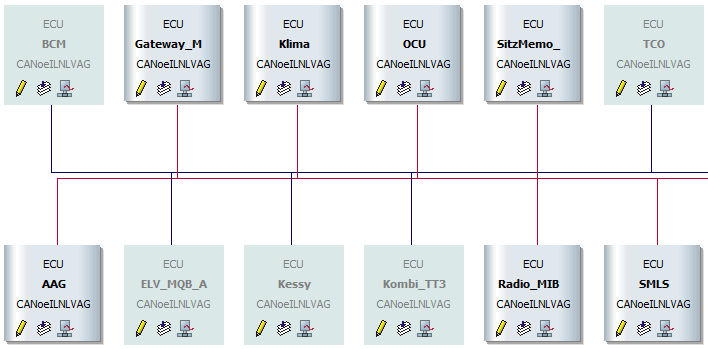
\includegraphics[width=\textwidth]{rbs_ausschnitt}
    \caption{Auschnitt der RBS Übersicht}
    \label{fig:rbs}
\end{figure}

Die Restbussimulation bietet noch weitere interessante Möglichkeiten. Abbildung \ref{fig:rbs} zeigt einen Ausschnitt der Simulationsübersicht in Vector CANoe. Hier lassen sich alle Steuergeräte ein- und ausschalten. Hierdurch kann eine beliebige Kombination von Hardware getestet werden, während der Rest per Software simuliert wird. Dabei können einzelne Signale von Hand ausgelöst und deren Werte umgestellt werden. Die Kommunikation zur Hardware wird dabei durch einen USB zu CAN Adapter von Vector realisiert.










%%%%%%%%%%%%%%%%%%%%%%%%%%%%%%% Entwicklung der AUTOSAR Anwendung %%%%%%%%%%%%%%%%%%%%%%%%%%%%%%%%%%
\section{Entwicklung der AUTOSAR Anwendung}
\label{sec:entwicklung_autosar}
Ziel der AUTOSAR-Komponente ist die Kommunikation mit, und das Befehle Empfangen von, der steuernden Komponente die im nächsten Kapitel entwickelt wird. Zur Realisierung der Kommunikation wird die Botschaft APP\_01 verwendet. Die darin enthaltenen Signale sind in Tabelle \ref{tab:App_Botschaft} zu sehen. Die Botschaft verwendet die ID 0x742, hat eine Länge von 4 Byte, und wird mit einer Zykluszeit von 100 ms gesendet.

\begin{table}[ht]
    \centering
    \begin{tabular}[h]{l c c c}
        Name & Byte & Bit & Länge\\
        \toprule
        APP\_Blinker\_li        & 1 &  0  & 1\\
        APP\_Blinker\_re        & 1 &  1  & 1\\
        APP\_Lichthupe          & 1 &  2  & 1\\
        APP\_Fernlicht          & 1 &  3  & 1\\
        APP\_Demo0              & 2 &  0  & 1\\
        APP\_Demo0\_Peridoe\_li & 3 &  0  & 4\\
        APP\_Demo0\_Periode\_re & 3 &  4  & 4\\
        APP\_Demo1              & 4 &  0  & 1\\
        APP\_Demo1\_Periode     & 4 &  4  & 4\\
        \bottomrule
    \end{tabular}
    \caption{Signale der Botschaft APP\_01}
    \label{tab:App_Botschaft}
\end{table}

Hierbei bieten die ersten vier Signale direkten Zugriff auf die entsprechenden Funktionen des BCM. Die restlichen Signale werden verwendet um zwei Demo-Modi anzusteuern. Diese sollen verdeutlichen, dass durch die Kommunikations-Kette, Python-AUTOSAR-BCM, eine Entkopplung der Funktionalität erreicht wird. So kann die steuernde Komponente zwar über die Botschaft einen Befehl senden, jedoch nicht direkt die Hardware beeinflussen. Dies übernimmt die AUTOSAR-Komponente und wirkt damit als Puffer zwischen Anwender und Hardware.

\begin{figure}[ht]
    \centering
    \resizebox{\linewidth}{!}{\input{./images/SMLS_Modell.dia}}
    \caption{Entwickeltes AUTOSAR Modell}
    \label{fig:smls_modell}
\end{figure}

Das gesamte System Modell ist in Abbildung \ref{fig:smls_modell} zu sehen. Auf der rechten Seite ist die steuernde Komponente, SWC\_APP, dargestellt. Diese ist in Python realisiert und nutzt den VCAN. Die Software Komponente SWC\_BCM stellt die ECU-Hardware dar. Obwohl beide Komponenten nicht mittels AUTOSAR realisiert werden, sind sie im Modell nötig, um die entsprechenden Ports zu definieren. Die hier erstellte AUTOSAR-Komponente ist als SWC\_SMLS im Modell sichtbar. Die Botschaften Licht\_vorne\_01 und Klemmen\_Status\_01 werden verwendet um den aktuellen Status anzeigen zu können. Die letzte verbleibende Botschaft, SMLS\_01, beinhaltet die Steuer-Signale vom SMLS zum BCM hin.

Auch die nötige CAN-Datenbank in Form einer .dbc-Datei entspricht dem Modell. Hier sind die ECUs und Botschaften ebenfalls nachgebildet. Ein besonderes Augenmerk ist dabei auf das Layout der Signale innerhalb der Botschaften zu legen. Sowohl die .dbc-Datei, als auch das SystemDesk Projekt, sowie die daraus resultierende .arxml-Datei sind auf der beigelegten CD zu finden.

Die ECU-Konfiguration mittels EB tresos wird nach den üblichen Verfahren durchgeführt. Dabei wurden als Grundlage der von EB durchgeführte Workshop, sowie die Unterlagen zur AUTOSAR-Lehrveranstaltung an der Ostfalia aus dem Wintersemester 2012/2013 genutzt. Die einzelnen Schritte zur Konfiguration der ECU sollen an dieser Stelle nicht aufgeführt werden, da diese in den genannten Dokumenten umfangreich erläutert sind. An dieser Stelle ist zu erwähnen, dass die ECU-Konfiguration mehr Zeit in Anspruch genommen hat, als zu Beginn des Projektes geplant. Dies folgt vor allem aus der häufig nötigen und langwierigen Fehlersuche.

\begin{lstlisting}[frame=single, language=C, basicstyle=\footnotesize, caption={Implementation der Runnable}, label={lst:headlight_final}]
void SWC_SMLS_R_SMLS (void) {
  init_iwrite_vars();
  read_values();

  if (DE_APP_Demo0) {
    /* run demo 0 */
  } else if (DE_APP_Demo1) {
    /* run demo 1 */
  } else if (DE_APP_Fernlicht || DE_APP_Lichthupe || DE_APP_Blinker_re || DE_APP_Blinker_li) {
    Rte_IWrite_R_SMLS_P_SMLS_01_DE_BH_Fernlicht(DE_APP_Fernlicht);
    Rte_IWrite_R_SMLS_P_SMLS_01_DE_BH_Lichthupe(DE_APP_Lichthupe);
    Rte_IWrite_R_SMLS_P_SMLS_01_DE_BH_Blinker_li(DE_APP_Blinker_li);
    Rte_IWrite_R_SMLS_P_SMLS_01_DE_BH_Blinker_re(DE_APP_Blinker_re);	
  }

  calc_crc();
  Rte_IWrite_R_SMLS_P_SMLS_01_DE_SMLS_01_BZ(bz_counter);
  increment_bz();	
}
\end{lstlisting}

Die Implementation des Kernelements der AUTOSAR-Anwendung, die Runnable, ist in Listing \ref{lst:headlight_final} aufgeführt. Dabei ist der Code der Übersicht halber gekürzt. Der komplette Quellcode ist auf der beigelegten CD enthalten. Zeile eins des Listings zeigt die Signatur der Runnable. Diese ist durch die RTE fest definiert. Die Zeilen zwei und drei enthalten Aufrufe von Initialisierungsfunktionen. Diese lesen alle aktuellen Werte der CAN-Botschaften ein, und speichern diese in Variablen. Die eigentliche Funktionalität ist in den Zeilen 5 bis 14 enthalten. Hier wird aufgrund der verschiedenen Modi eine bestimmte Aktion ausgeführt. So werden in den Zeilen 10 bis 13, die APP-Signale direkt auf SMLS-Signale geschrieben, falls kein Demo-Modus aktiv ist.

Zum Schluss der Funktion, wird in den Zeilen 16 bis 18, die endgültige Botschaft gesendet. Dazu wird zuerst der CRC durch eine Lookup-Table bestimmt, und anschließend der Botschaftenzähler gesendet und inkrementiert. Das Nutzen des impliziten Sendens, sichtbar durch die \texttt{IWrite}-Methodenaufrufe, führt dazu, dass die eigentliche Botschaft erst gesendet wird, sobald die Runnable vorbei ist. Bis dahin werden die geschriebenen Werte zwischengespeichert. Das ist nötig, da ansonsten bei jedem Sende-Aufruf die gesamte Botschaft gesendet wird, obwohl noch nicht alle Signale gesetzt wurden.









%%%%%%%%%%%%%%%%%%%%%%%%%%%%%%% Entwicklung der steuernden Komponente %%%%%%%%%%%%%%%%%%%%%%%%%%%%%%%%%%
\section{Entwicklung der steuernden Komponente}
\label{sec:entwicklung_vcan_app}
Die steuernde Komponente basiert auf der VCAN-API und bietet eine Oberfläche, mit deren Hilfe sich die Demofunktionen leicht aktiveren lassen. Zudem werden aktuelle Statusinformationen vom CAN-Bus übersichtlich dargestellt. 

\begin{figure}
    \centering
    \begin{subfigure}[b]{0.59\textwidth}
        \centering
        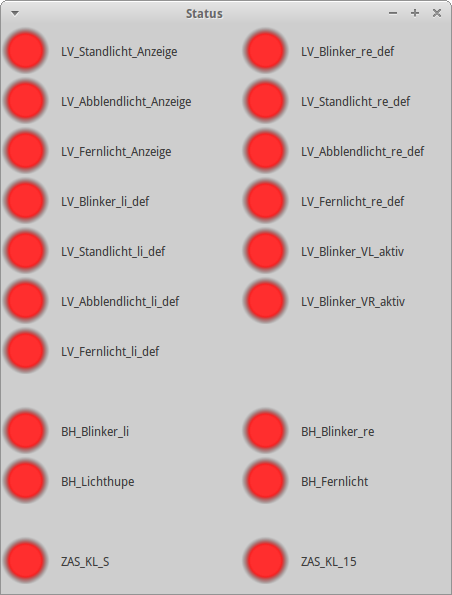
\includegraphics[width=\textwidth]{vcan_app_status}
        \caption{Status-Fenster}
        \label{fig:vcan_app_status}
    \end{subfigure}
    \begin{subfigure}[b]{0.39\textwidth}
        \centering
        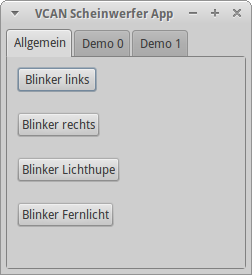
\includegraphics[width=\textwidth]{vcan_app_control}
        \caption{Kontroll-Fenster}
        \label{fig:vcan_app_control}
    \end{subfigure}
    \caption{Oberfläche der VCAN-Applikation}
    \label{fig:vcan_app}
\end{figure}

Die Oberfläche der in diesem Projekt entwickelten Anwendungen besteht aus zwei Fenstern. Sie ist mittels wxPython realisiert, da dieses Plattformübergreifend ohne Anpassungen unterstützt wird. Das in Abbildung \ref{fig:vcan_app_status} zu sehende Status-Fenster, stellt die Informationen der verwendeten CAN-Botschaften\footnote{\texttt{Licht\_vorne\_01}, \texttt{SMLS\_01} und \texttt{Klemmen\_Status\_01}} in einer übersichtlichen Darstellung dar.

Abbildung \ref{fig:vcan_app_control} zeigt das Kontrollfenster. Dieses bietet direkten Zugriff auf alle Signale der \texttt{APP\_01} Botschaft. Zudem können die zwei Demomodi über die Reiter angesprochen werden.















%%%%%%%%%%%%%%%%%%%%%%%%%%%%%%% Analyse des Fallbeispiels %%%%%%%%%%%%%%%%%%%%%%%%%%%%%%%%%%
\chapter{Analyse des Fallbeispiels}
\label{sec:Beispiel_Analyse}
Dieses Kapitel betrachtet die Ergebnisse des Fallbeispiels. Dabei wird im nächsten Kapitel auf die Praxisrelevanz der Techniken eingegangen. Anschließend wird das Zeitverhalten des VCAN Systems untersucht. Dies ist vor allem im Hinblick auf die Echtzeitfähigkeit interessant. Ein weiteres, in der Praxis relevantes Thema, ist die Sicherheit. Diese wird anhand dieses Fallbeispiels im darauf folgenden Kapitels betrachtet.



%%%%%%%%%%%%%%%%%%%%%%%%%%%%%%% Relevanz für die reale Projekte %%%%%%%%%%%%%%%%%%%%%%%%%%%%%%%%%%
\section{Relevanz für reale Projekte}
\label{sec:Relevanz}
Die Zukunft der Elektronik in der Automotiveindustrie ist stark durch Infotainment und Fahrerassistenzsysteme geprägt. Diese Systeme liegen zwischen zwei Ebenen. Zum Einen die Lowlevel Ebene, die die Anbindung an die Fahrzeughardware bietet und dem klassischen Modell entspricht, und zum Anderen eine Highlevel Ebene, die eine Anbindung an Car2X Netzwerke und ähnliches bietet. Genau dieser immer größer werdende Bereich kann von den Vorteilen der embedded Virtualisierung profitieren. Wie in den bisherigen Kapiteln klar geworden ist, handelt es sich um eine ausgereifte Technik. Es existieren schon einige Hypervisoren, die auch zum Beispiel in der Mobilfunkbranche bereits eingesetzt werden. Auch die Avionik hat die Vorteile bereits seit einigen Jahren erkannt und setzt die Techniken erfolgreich ein.

Ein wichtiges Argument für den Einsatz von Virtualisierung sind die Kosten. Dies soll im Folgenden an einem Beispiel näher untersucht werden. Das Beispiel ist dabei nicht vollständig repräsentativ und soll lediglich den Grundgedanken aufzeigen. Dementsprechend ist die Wahl der Hardware relativ frei und nicht auf eine konkrete Anwendung bezogen.

Angenommen wird ein System bestehend aus vier ECUs. Die Steuergeräte basieren jeweils auf einem LPC4310 Microcontroller von NXP. Diese werden aktuell mit etwa 10 \$ pro Stück gelistet und bieten jeweils eine Rechenleistung von 200 MHz. Nun werden diese ECUs mittels Virtualisierung vereint. Hier wird als Zielsystem ein Nvidia Tegra 3 betrachtet, der zur Zeit für etwa 20 \$ erhältlich ist. Dieser bietet gleich vier Kerne mit je 1,6 GHz Leistung und einen Kern mit 500 MHz Leistung. Hier zeichnet sich bereits eine mögliche Struktur des Zielsystems ab. 

Der langsame Kern kann dediziert den Hypervisor übernehmen, während die anderen vier Kerne die Funktionalität der ECUs übernehmen. Da für jede ECU nun ein vielfaches der Leistung vorhanden ist, sollte die Echtzeitfähigkeit kein Problem darstellen. Mit dieser Umstellung werden die Kosten in diesem Beispiel von 40 \$ auf 20 \$ halbiert. Hinzukommen ebenso Ersparnisse hinsichtlich der eingesetzten Boards beziehungsweise Peripherie, sowie unter Umständen ein vereinfachter Kabelbaum. Entsprechende Kosten werden hier jedoch nicht betrachtet, da diese nicht einfach einzuschätzen sind. Ebenso wird ein nötiger Integrationsaufwand nicht betrachtet. Trotz dieser Einschränkungen ist eine Richtung zu erkennen: Die Kosten sowie die Hardwarekomplexität des Systems kann verringert werden.

Ebenso kann die Umsetzung der funktionalen Sicherheit nach ISO 26262 von eingebetteter Virtualisierung profitieren. Virtuelle Maschinen trennen dabei Teilsystem ab und können die Sicherheitsbetrachtung auf mehrere Domänen aufteilen. Einzig der Hypervisor, als zentrales Element, erhöht die Komplexität des Systems und Bedarf umfangreicher Sicherheitsuntersuchung. Anschließend ist jedoch ein Bausatzsystem vorstellbar, in dem Funktionalität in virtuellen Maschinen gekapselt wird und anschließend diese als abgesicherte und getestete Bausteine eingesetzt werden. Integrationstests sind jedoch auch hier nötig.

Der Bereich des Testens kann ebenfalls durch Virtualisierung erweitert werden. Da eine virtuelle Maschine auf einer abstrakten Ebene ausgeführt wird, ist es auch mögliche diese portabel zu gestalten, um so sowohl auf der embedded Hardware als auch auf einer Testhardware lauffähig zu sein. So ist es denkbar das Produktivcode, gekapselt in einer VM, auch im Testeinsatz Verwendung findet und somit als Restbussimulation für echte Hardware dient.

Ein ähnliches Konzept wird auch durch EB tresos WinCore erreicht. Da durch EB tresos sowohl Projekte für Windows, als auch für embedded Plattformen erstellt werden können, kann der Programmcode zum Großteil übernommen werden. Jedoch ist hier eine umfangreiche Konfiguration der RTE und der restlichen Module nötig. Daher eignet sich WinCore vor allem für die ersten Phasen eines Projektes, sowie die Lehre. Da die Applikation auf üblichen Betriebssystemen und Rechnern lauffähig ist, werden die Komplikation bei der Nutzung einer embedded Plattform vermieden beziehungsweise verschoben.

Vor allem der Einsatz des VCANs erleichtert viele Arbeiten und erste Tests. Da hier auf Ethernet, und damit auf eine ausgereifte und weit verbreitete Technik gesetzt wird, ist der Zugriff sehr einfach zu realisieren. In diesem Projekt wurde auf Python gesetzt. Aber auch praktisch jede andere Programmierumgebung ist denkbar, da der Zugriff auf TCP-Sockets nahezu immer möglich ist. Und da der Umgang mit Highlevel-Umgebungen dieser Art relativ einfach ist, ist eine erweiterte Funktionalität vorstellbar. Dies reicht vom auslesen einer Konfigurationsdatei um Stimuli einzurichten, bis hin zu einer Weboberfläche um den Zugriff auf den gesamten Bus zu erlauben. Auch eine Anbindung an MATLAB-Modelle ist möglich.



%%%%%%%%%%%%%%%%%%%%%%%%%%%%%%% Benchmark und Betrachtung der Echtzeitfähigkeit %%%%%%%%%%%%%%%%%%%%%%%%%%%%%%%%%%
% 
\section{Benchmark und Betrachtung der Echtzeitfähigkeit}
\label{sec:Benchmark}
Dieses Kapitel betrachtet das Zeitverhalten des VCAN. Dabei wird versucht eine Aussage zur Echtzeitfähigkeit zu machen. Die Analyse beschränkt sich auf einige wenige Anwendungsfälle. Alle Kombinationen aus Betriebssystem, Netzwerk-, CPU-Last und anderen Faktoren zu testen ist nicht praktikabel.

Allgemein ist zu sagen, dass Ethernet nicht für harte Echtzeitanforderungen geeignet ist. Da der VCAN jedoch vor allem für die Evaluation und einfache Tests ausgelegt ist, lässt sich Ethernet an dieser Stelle trotzdem gut einsetzen. Die Latenz kann dabei verringert werden, indem die Netzwerklast verringert, sowie die Netzwerkarchitektur vereinfacht wird. Das bedeutet, dass die Kommunikation das Testsystems in einem separaten Teilnetz stattfindet, auf das möglichst keine anderen Geräte zugreifen können. 

Zur Analyse des Zeitverhaltens wurde eine Benchmark Anwendung entwickelt. Diese startet ein VCAN-Gateway und speichert die Zeiten eingehender Botschaften. Diese können anschließend ausgewertet werden. Abbildung \ref{fig:timinganalyse} zeigt die Ergebnisse zweier Testreihen als Boxplots. Dabei beträgt die Größe der Stichproben jeweils 1\,000 Botschaften.

\begin{figure}
    \centering
    \begin{subfigure}[b]{0.49\textwidth}
        \centering
        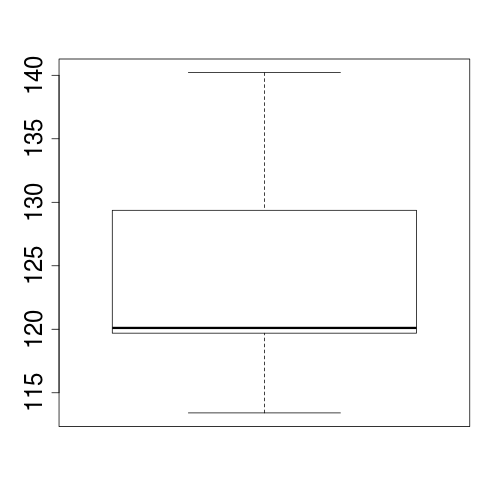
\includegraphics[width=\textwidth]{boxplot_as}
        \caption{Zeitverhalten AUTOSAR}
        \label{fig:boxplot_as}
    \end{subfigure}
    \begin{subfigure}[b]{0.49\textwidth}
        \centering
        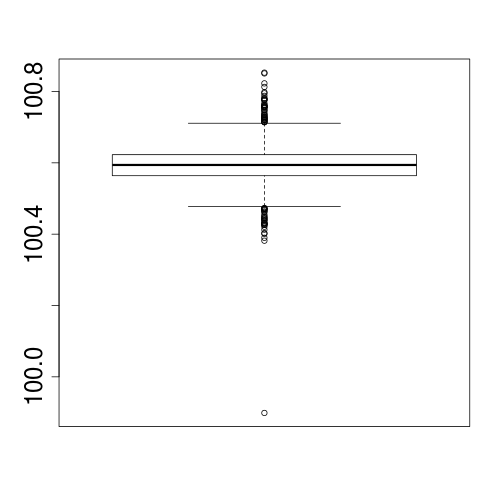
\includegraphics[width=\textwidth]{boxplot_vcan}
        \caption{Zeitverhalten VCAN-API}
        \label{fig:boxplot_vcan}
    \end{subfigure}
    \caption[Zeitanalyse des VCAN als Boxplots]{Zeitanalyse des VCAN als Boxplots (Angaben in ms)}
    \label{fig:timinganalyse}
\end{figure}

Wie in Abbildung \ref{fig:boxplot_as} zu erkennen ist, liegen die Werte etwa im Bereich von 20 ms um den Median 120 ms herum. Diese Streuung ist für die vorgesehenen Anwendungen durchaus akzeptabel. Der Mittelwert der Messungen scheint jedoch von der Netzwerkarchitektur abzuhängen. So wurden diese Werte im FH-Netz gemessen. In zwei anderen Netzwerken konnten Durchschnitts werden von 110 ms sowie 130 ms festgestellt werden. Die Ursache dieser Abweichung ist nicht geklärt. Da es sich jedoch um einen relativ konstanten Wert handelt, kann dieser durch Maßnahmen innerhalb des System-Modells oder der RTE-Konfiguration ausgeglichen werden.

Zudem wurde während des Projektes eine Eigenheit des WinCore VCAN beobachtet, die jedoch in dieser Auswertung nicht reproduziert werden konnte. Hierbei kam es immer wieder zu langen Pausen, gefolgt von Sendehäufungen. Dies führt zu einer stark erhöhten Standardabweichung.

Abbildung \ref{fig:boxplot_vcan} zeigt die Ergebnisse der Analyse bei Benutzung der VCAN-API. Hier ist zu erkennen, dass eine Genauigkeit von etwa einer Millisekunde möglich ist. Lediglich einzelne Ausreißer, in diesem Fall nur einer, weichen einige Millisekunden vom gewünschten Wert ab.

Tabelle \ref{tab:jitter_statistik} führt die Eigenschaften der Stichproben auf. Auch hier zeigen sich die beschriebenen Ergebnisse. Die Standardabweichung beim Einsatz der VCAN-API beträgt lediglich 0.1 ms, während diese beim Einsatz von AUTOSAR 4.8 ms beträgt. Damit sind beide Werte im akzeptablen Bereich um weiche Echtzeit für die vorgesehenen Anwendungen zu ermöglichen.

\begin{table}[ht]
    \centering
    \begin{tabular}[h]{r  r r}
            & Stichprobe AUTOSAR & Stichprobe VCAN\\
        \toprule
        Durchschnitt        & 122.9 ms & 100.0 ms\\
        Median              & 120.1 ms & 100.0 ms\\
        Maximal Wert        & 140.2 ms & 100.3 ms\\
        Minimal Wert        & 113.4 ms & 97.2 ms\\
        25\% Quantil        & 119.7 ms & 100.0 ms\\
        75\% Quantil        & 129.4 ms & 100.0 ms\\
        Standardabweichung  & 4.8 ms & 0.1 ms\\
        \bottomrule
    \end{tabular}
    \caption{Statistische Eigenschaften der Stichproben}
    \label{tab:jitter_statistik}
\end{table}

Da die Implementation des WinCore nicht offen liegt, lässt sich das Zeitverhalten hier nicht verbessern. Beim Einsatz der VCAN-API sind jedoch einige Möglichkeiten denkbar. Bisher wurden wxPython und pygame eingesetzt um konstante Timer zu erhalten. Diese sorgen dafür, dass die Ausführungszeit nicht zur Wartezeit hinzukommen. Dabei konnten mittels pygame zuverlässig Sendezyklen bis 1 ms getestet werden. Damit ist der Bereich üblich genutzter Zeiten abgedeckt. Um den Jitter noch weiter zu verringern ist es denkbar \emph{High Precision Event Timer} zu nutzen. Diese können theoretisch Zeiten bis 100 ns auflösen.



%%%%%%%%%%%%%%%%%%%%%%%%%%%%%%% Sicherheit bei Embedded Virtualisierung %%%%%%%%%%%%%%%%%%%%%%%%%%%%%%%%%%
\section{Sicherheitsbetrachtung}
\label{sec:Sicherheit_Beispiel}
Da es sich bei dem Beispielsystem lediglich um eine Scheinwerfersteuerung handelt, ist Sicherheit kein besonders kritisches Thema. Die Folgenden Punkte sind jedoch genauso auf jedes andere System anwendbar und sind somit relevant. Bei dem Begriff \emph{Sicherheit} müssen zwei Arten unterschieden werden. Zum Einen die Angriffssicherheit, die einen böswilligen Angreifer annimmt, und zum Anderen die Betriebssicherheit, bei der ein technischer Ausfall betrachtet wird. Der in diesem Projekte eingesetzt VCAN hat in einigen Tests eine gewisse Fehleranfälligkeit gezeigt. Das fehlerhafte Setzen einzelner Bits kann zum Absturz der AUTOSAR Komponenten führen. Da der VCAN jedoch, in dieser Form, nur für Tests und Evaluation zum Einsatz kommt, sind diese Fehler nicht relevant für die spätere Sicherheit des Autos.

\paragraph{Angriffssicherheit}
Das hier betrachtete System bietet im Prinzip die selben Angriffsmöglichkeiten wie klassische Systeme. Sobald ein physischer Zugriff auf das System möglich ist, existieren eine Reihe von Möglichkeiten das System zu kompromittieren. Dabei zeigt ein virtualisiertes System keine Vorteile einem klassischen System gegenüber. Ein zentraler Hypervisor bietet zwar die Möglichkeit die Integrität der virtuellen Maschinen zu überprüfen, jedoch kann auch dieser selbst kompromittiert sein. Seitenkanalangriffe\footnote{Seitenkanalangriffe bezeichnen eine Gruppe von Angriffszenarien, bei denen das System von außen analysiert wird. Hierbei kann zum Beispiel anhand des Energieverbrauchs auf ausgeführte Befehle geschlossen werden.} könnten durch die erhöhte Komplexität des Systems erschwert werden. Eine Verhinderung dieser ist jedoch wahrscheinlich nicht möglich.

Ein weiterer Angriffsweg ist durch eine Internet- beziehungsweise Netzwerkanbindung gegeben. Diese erfahren eine immer größere Verbreitung, durch Car2Car-Kommunikation und das Nutzen des Internets für zum Beispiel Stauinformationen. Hier besteht eine durchaus große Gefahr. Eine kompromittierte VM kann durch eventuelle Sicherheitslücken im Hypervisor das ganze System lahmlegen. Daher muss dieser mit großer Sorgfalt entwickelt werden. Die Folgen einer Übernahme sind jedoch bei einem virtualisierten System nicht umfangreicher als bei einem klassischen System. In beiden Fällen könnte ein kompromittiertes Steuergerät den gesamten Bus lahmlegen, indem dauerhaft Nachrichten gesendet werden.

\paragraph{Betriebssicherheit}
Die Umstellung auf eine virtualisierte Umgebung bedeutet auch die Umstellung von einem verteilten System, hin zu einem vereinten System. Das bedeutet das weniger Hardware Redundanz vorhanden ist, und somit ein Ausfall der Hardware zum Verlust von mehr Funktionalität führt. Damit stellt die Hardware des Hosts, ebenso wie der Hypervisor, einen \emph{single point of failure} dar. Damit besitzt ein virtualisiertes System einen relevanten Nachteil. Da jedoch die Kosten für ein solches System niedriger Ausfallen können, kann zusätzlicher Aufwand betrieben werden, um zuverlässigere Bauteile einzusetzen und die Sicherheitsüberprüfungen auszuweiten. Ob sich diese Rechnung für konkrete Projekt lohnt, muss im Einzelfall entschieden werden. Ein zentraler Hypervisor bietet jedoch auch einige Möglichkeiten. So kann eben hier eine Diagnose stattfinden, um die Zuverlässigkeit der virtuellen Maschinen zu gewährleisten. 


\paragraph{Absicherung der Verbindung}
Ein weiteres Konzept. dass vor allem bei Verbindungen zum Internet relevant ist, ist das Signieren und Verschlüsseln von Nachrichten. Dabei wird vor allem versucht die Integrität und Authentizität zu gewährleisten. Somit kann zum Beispiel das Einschleusen veränderter Kartendaten verhindert werden. Eine im Internet weit verbreitete Technik hierfür ist SSL. Die dabei verwendeten Algorithmen, wie zum Beispiel RSA oder MD5, sind jedoch in üblichen Automotiveanwendungen nicht vorhanden. Daher müssen diese beim Nutzen offener Netzwerke wie dem Internet oder Car2Car-Kommunikation implementiert werden. AUTOSAR sieht ab Version 4.0 einen \emph{Crypto Service Manager} vor. Dieser kann Techniken wie MD5, SHA1 oder weitere anbieten. Es wird jedoch im Standard nicht vorgegeben, welche dieser Techniken implementiert werden müssen. Daher ist hier im Einzefall die Verfügbarkeit genau zu prüfen.

Auch mittels Virtualisierung lässt sich ein ähnliches Konzept aufbauen. Dabei kann eine virtuelle Maschine jegliche Kryptographische Verfahren implementieren und diese anderen Instanzen zu Verfügung stellen. Dadurch beschränken sich alle sicherheitskritischen Komponenten, wie zum Beispiel Zertifikate, Schlüssel und Algorithmen, auf eine virtuelle Maschine. Diese kann entsprechend vor Angriffen gesichert werden um so einen Schutz zu gewährleisten. Eine Übernahme dieser Instanz würde hingegen jedoch auch einen Totalausfall der gesicherten Verbindungen bedeutet. Daher muss auch hier zwischen einer verteilten und einer vereinigten Architektur entschieden werden.








%%%%%%%%%%%%%%%%%%%%%%%%%%%%%%% Zusammenfassung %%%%%%%%%%%%%%%%%%%%%%%%%%%%%%%%%%
\chapter{Fazit und Ausblick}
\label{sec:FazitAusblick}
Zusammenfassend lässt sich sagen, dass die Virtualisierung ein interessantes und ausgereiftes Konzept darstellt, dass durchaus auch in der Welt der eingebetteten Systeme Anwendung finden kann. Zwar wird die Systemkomplexität durch den Einsatz von Virtualisierung erhöht, jedoch wird gleichzeitig auch durch die starke Abstraktion und strikte Trennung ein alternatives Entwicklungskonzept ermöglicht. Hierin lassen sich Teilsysteme Bausteinartig einsetzen, und das System in einem Top-Down-Verfahren entwerfen. Eine konkrete Kosten-Nutzen-Rechnung muss jedoch in jedem Projekt einzeln erfolgen, da eine allgemeine Aussage dazu in dieser Arbeit nicht möglich ist.

Die in diesem Projekt eingesetzte AUTOSAR-Distribution WinCore, sowie der darin integrierte VCAN, sind sehr gut in der Lehre, sowie in einer ersten Evaluationsphase zu nutzen. Bei längerer Benutzung zeigt sich jedoch die Instabilität als kritische Eigenschaft, sodass ein Produktiveinsatz in dieser Weise nicht möglich ist. Beim VCAN handelt es sich um eine einfache und offene Möglichkeit, in die Kommunikation des Systems einzugreifen, um somit eine Restbussimulation sowie manuelle Tests schnell zu ermöglichen.

An dieser Stelle zeigt sich auch Potential für zukünftige Projekte. Sollte der VCAN auch weiter eingesetzt werden, bietet es sich an, die Integration der Kommunikationsmatrix, sowie der Systembeschreibung zu realisieren. Hierdurch wäre eine Übersichtliche Nutzung, sowie eine schnelle Einrichtung einer einfachen Restbussimulation möglich. Da die in dieser Arbeit erstellten VCAN-API offen gehalten ist, sind entsprechende Anpassungen nach kurzer Einarbeitungszeit implementierbar.

% TODO: 
% - AUTOSAR meiner Meinung nach nicht toll!
%   - Idee gut und nötig
%   - Jedoch von zu vielen beeinflusst
%   - Zu konkret
%   - sollte einfacher und allgemeiner gehalten sein
% - VCAN ebenfalls eine gute Idee, jedoch auch nicht perfekt umgesetzt














%%%%%%%%%%%%%%%%%%%%%%%%%%%%%%%%%%% Anhang %%%%%%%%%%%%%%%%%%%%%%%%%%%%%%%%%

\appendix
\part*{Anhang}

% This file contains sensitive information that is not shared on GitHub!!!
\InputIfFileExists{appendix_nda}{}






%%%%%%%%%%%%%%%% VCAN-API %%%%%%%%%%%%%%%%%%%%
\chapter{VCAN-API}
\label{sec:vcan_api}
Dieses Kapitel beschreibt die im Laufe des Projektes erstellte Software zur Kommunikation per virtuellem CAN. Alle Informationen über das Protokoll wurden per Reverse Engineering ermittelt.
% TODO:


\section{Protokoll}
\label{sec:vcan_protokoll}
% TODO:
% Protokoll, duh?!



\section{Projekt Struktur}
\label{sec:vcan_struktur}
% TODO:
% Dateien, Klassen
% Abhängigkeiten
\begin{description}
    \apiitem{./vcan\_api/}
    Dieses Verzeichnis enthält die gesamte VCAN-API.
    \begin{description}
        \apiitem{./vcan\_api/\_\_init\_\_.py}
        VCAN-API Python Pyackage.
        \apiitem{./vcan\_api/PCANBasic.py}
        API zur Nutzung des PEAK-PCAN-USB-Adapters. Diese Datei stammt von PEAK.
        \apiitem{./vcan\_api/vcan\_client.py}
        Enthält die Klasse VCANClient.
        \apiitem{./vcan\_api/vcan\_config.py}
        Enthält die Klasse VCANConfig.
        \apiitem{./vcan\_api/vcan\_config.xsd}
        XML-Schema für Firewall-Konfigurationen.
        \apiitem{./vcan\_api/vcan\_exception.py}
        Enthält die Klasse VCANException.
        \apiitem{./vcan\_api/vcan\_gateway.py}
        Enthält die Klasse VCANGateway.
        \apiitem{./vcan\_api/vcan\_message.py}
        Enthält die Klasse VCANMessage und einige Konstanten um diese zu Nutzen.
    \end{description}
    \apiitem{./gateway.py}
    Ein simples Gateway mit grafischer Oberfläche.
    \apiitem{./gateway\_rules.xml}
    Eine Beispiel-Konfiguration der im Gateway eingebauten Firewall-Regeln.
    \apiitem{./sample\_*.py}
    Verschiedene Python-Beispiele, die die VCAN-API nutzen.
\end{description}


\section{Gateway API}
\label{sec:vcan_gateway_api}

% class VCANGateway
\begin{description}
    \apiitem{class VCANGateway(receive\_callback=None, connection\_callback=None)}
    Das Gateway nimmt Verbindungen von Clients entgegen und verteilt eingehende Botschaften an alle angemeldeten Clients weiter.
    \begin{description}
        \apiitem{start\_gateway(host='127.0.0.1', port=10020, rulesfile='')}
        Startet das Gateway auf IP \texttt{host} und dem Port \texttt{port}. Auf dem ausführenden Rechner muss ein Netzwerk-Interface mit der entsprechenden IP existieren. Der Port darf nicht durch eine andere Anwendung belegt sein. Optional kann eine Regeldatei angegeben werden um Firewall-Regeln zu definieren. Dies ist noch experimentell.
        \apiitem{stop\_gateway()}
        Stoppt das Gateway wieder. Anschließend kann mittels der \texttt{start\_gateway} Methode wieder gestartet werden. Es werden jedoch alle Verbindungen getrennt, und die Host IP muss ein weiteres mal angegeben werden.
        \apiitem{connect\_other\_gateway(host, port=10020)}
        Ein Gateway kann sich zu einem anderen Gateway verbinden um ein Netz zu bilden. Das Ziel-Gateway muss unter der IP \texttt{host} und dem Port \texttt{port} erreichbar sein. Diese Methode ist hilfreich, wenn zum Beispiel eine Firewall eingehende Verbindungen verbietet oder ein Gateway unter Linux mit einem Windows-Gateway verbunden wird, um den PCAN nutzen zu können.
        \apiitem{pcan\_init()}
        Initialisiert den ersten gefundenen PEAK-PCAN USB-Dongle mit einer Baud-Rate von 500kbaud. Das gwählte USB-Interface und die Baud-Rate können zur Zeit nur im Code geändert werden. PCAN Support ist im Moment nur unter Windows vorhanden und wird ansonsten durch eine VCANException markiert.
        \apiitem{pcan\_uninit()}
        Deinitialisiert den PEAK-PCAN USB-Dongle.
    \end{description}
\end{description}

% class VCANConfig
\begin{description}
    \apiitem{class VCANConfig(rulesfile)}
    Diese Klasse wird verwendet um Firewall-Regeln im Gateway zu implementieren. Hierzu wird eine XML-Datei mit Regeln übergeben. Diese Datei muss dem beiligenden Schema \texttt{vcan\_config.xsd} entsprechen. Das Gateway ist dafür verantwortlich die entsprechenden Überprüfungen beim Senden und Empfangen durchzuführen.
    \begin{description}
        \apiitem{is\_send\_allowed(ip, can\_id)}
        Überprüft ob die IP \texttt{ip} eine Botschaft mit der ID \texttt{can\_id} senden darf. Gibt True zurück falls erlaubt, und False falls verboten.
        \apiitem{is\_receive\_allowed(ip, can\_id)}
        Überprüft ob die IP \texttt{ip} eine Botschaft mit der ID \texttt{can\_id} empfangen darf. Gibt True zurück falls erlaubt, und False falls verboten.
    \end{description}
\end{description}

% class VCANException
\begin{description}
    \apiitem{class VCANException(value)}
    Exception der VCAN-API. Wird beim Gateway verwendet, falls die PCAN-Verbindung nicht initialisiert werden kann.
\end{description}




\section{Client API}
\label{sec:vcan_client_api}

% class VCANClient
\begin{description}
    \apiitem{class VCANClient(q\_length=1024)}
    Diese Klasse kann verwendet werden, um Zugriff auf den VCAN zu erhalten. Es bietet Funktionen um eine Verbindung aufzubauen und zu schließen. Außerdem können Botschaften empfangen und gesendet werden. Standardmäßig erfolgt das Empfangen auf Polling-Basis. Hierzu wird eine Queue der Länge \texttt{q\_length} angelegt. Der Anwender ist verantwortlich die eingehenden Daten häufig genug zu pollen. Alternativ kann für das Empfangen eine Callback-Funtion angegeben werden.
    \begin{description}
        \apiitem{connect(ip, port=10020, receive\_data=True, callback=None)}
        Verbindet den Client mit einem Gateway auf IP \texttt{ip} und Port \texttt{port}. Über den Schalter \texttt{receive\_data} kann das Empfangen von Botschaften deaktiviert werden. Der Parameter \texttt{callback} kann verwendent werden um eine Funktions-Referenz zu übergeben, die empfangene Botschaften direkt verarbeitet. Wirft \texttt{VCANException} falls keine Verbindung hergestellt werden kann.
        \apiitem{close(sleep\_time=0.5)}
        Schließt die aktuelle Verbindung. Der Parameter \texttt{sleep\_time} wird verwendet um nach dem Schließen der Verbindung einen Moment zu warten. Damit werden Eigenheiten des EB-Gateways und der AUTOSAR-Anwendungen ausgeglichen, da es ansonsten zu Fehlern kommen kann. Die Angabe erfolgt in Sekunden.
        \apiitem{get\_received\_item()}
        Gibt die älteste empfangene Botschaft zurück. Falls die Queue leer ist wird \texttt{None} zurückgegeben. Diese Methode muss im Polling-Betrieb häufig genug aufgerufen werden, um Daten-Verlust zu vermeiden.
        \apiitem{send(message, sleep\_time=0.2)}
        Sende die Botschaft \texttt{message} zum verbundenden Gateway. Die Botschaft kann sowohl als Binär-String, als auch als VCANMessage vorliegen. Der Parameter \texttt{sleep\_time} wird verwendet um Fehler zu vermeiden indem nach dem Senden ein Moment gewartet wird. Falls nur Applikation angebunden sind, die die VCAN-API nutzen kann dieser Wert auf 0 gesetzt werden. AUTOSAR-Applikation haben jedoch Probleme mit zu geringen Warte-Zeiten und können Botschaften verlieren oder sogar abstürzen. Die Angabe erfolgt in Sekunden. Falls der Client zu keinem Gateway verbunden ist, wird eine \texttt{VCANException} geworfer.
    \end{description}
\end{description}

% class VCANMessage
\begin{description}
    \apiitem{class VCANMessage()}
    Repräsentiert eine Botschaft in der VCAN-API. Der Konstruktur generiert eine leere Botschaft. Diese kann entweder über \texttt{set\_parameters()} von Hand mit Parametern gefüllt werden, oder über \texttt{parameters\_from\_string()} von einer eingehenden Nachricht aus einem Binär-String.
    \begin{description}
        \apiitem{set\_parameters(can\_id,  data, system, channel, dlc=None)}
        Setzt die Parameter der Nachricht entsprechend den Parametern. Parameter \texttt{can\_id} gibt die ID der Botschaft an. Die Nutzdaten sind werden in \texttt{data} erwartet und müssen als Liste übergeben werden. Die Parameter \texttt{system} und \texttt{channel} geben das entsprechende System und den Kanal an. Standard-Werte sind CAN und Kanal 0. Weitere Möglichkeiten sind in der Datei \texttt{vcan\_message.py} als Konstanten hinterlegt. Der letzte Parameter, \texttt{dlc}, gibt die Länge der Daten an. Falls \texttt{None} übergeben wird, wird die Länge des Daten-Arrays verwendet.
        \apiitem{parameters\_from\_string(m\_string)}
        Setzt die Parameter der Nachricht anhand des Binär-Strings \texttt{m\_string}. Diese entsprechen direkt dem TCP-Paket und können hierdurch in eine VCAN-API-konforme Form gebracht werden.
        \apiitem{to\_sendable\_string()}
        Wandelt die Botschaft in einen Binär-String um, der per TCP versendet werden kann.
    \end{description}
\end{description}

% class VCANException
\begin{description}
    \apiitem{class VCANException()}
    Exception der VCAN-API. Wird geworfen falls die Verbindung zu einem Gateway scheitert, oder eine Nachricht gesendet wird obwohl keine Verbindung besteht. Außerdem siehe \ref{sec:vcan_gateway_api}
\end{description}




\section{Beispiel Anwendungen}
\label{sec:vcan_beispiele}

















% Alles hier nach hat keine Nummerierung mehr...
\backmatter


\chapter{Beigelegte CD}
\label{sec:BeigelegteCD}
% TODO:
\begin{itemize}
    \item AUTOSAR Spezifikation
    \item Projektdaten
    \begin{itemize}
        \item CAN-Datenbank
        \item Systembeschreibung
        \item Tresos Konfiguration
        \item Quellcode AUTOSAR
        \item VCAN Applikation
    \end{itemize}
    \item Quellen
    \item VCAN-API
    \item VCAN Gateway
    \item XtratuM Projekt
\end{itemize}


%%%%%%%%%%%%%%%%%%%%%%% Erklärung und CD %%%%%%%%%%%%%%%%%%%%%%%%%%%%%
\chapter{Erklärung}
\label{sec:Erklärung}
Hiermit erkläre ich, dass ich die vorliegende Arbeit selbstständig und nur unter Verwendung der angegebenen Quellen und Hilfsmittel erstellt habe.
\vspace{2.5cm} \par
Wolfenbüttel, den % TODO


% Alle Einträge zum Glossar hinzufügen und Glossar/Akronymliste printen
\glsaddall
\printglossaries


%%%%%%%%%%%%%%%%%%%%%%%%%%%%%%% Bibliographie %%%%%%%%%%%%%%%%%%%%%%%%%%%%%%
% \setbibpreamble{Die Quellenangaben sind alphabetisch nach den Namen der Autoren sortiert.
% Bei mehreren Autoren wird nach dem ersten Autor sortiert.\par\bigskip\bigskip}

\nocite{*}

\begin{singlespace}
\bibliographystyle{natdin}	% alphadin, plaindin, abbrvdin, unsrtdin, natdin
					            % germbib: gerabbrv, geralpha, gerplain, gerunsrt, gerapali, gerxampl
                           		% plainnat, abbrvnat, unsrtnat
                           		% Am besten geeignet: natdin
                           		% oder was ist mit dinat
                           		% ???apalike???
\bibliography{literature}
\end{singlespace}
%%%%%%%%%%%%%%%%%%%%%%%%%%%%%%%%%%%%%%%%%%%%%%%%%%%%%%%%%%%%%%%%%%%%%%%%%%%%

\end{document}


